% ### PREAMBOLO ### %
\documentclass[italian, a4paper, twoside, titlepage, 10pt]{article} % Tipo di documento

% Margini (il bindingoffset � lo spazio per la rilegatura)
\usepackage[includehead, headheight=1.5cm, headsep=0.5cm, top=2.3cm, bottom=1.3cm, left=1.4cm, right=1.4cm, bindingoffset=0.3cm]{geometry}

\usepackage[breaklinks, colorlinks, linkcolor=blue]{hyperref} % Per gli hyperlink

\usepackage{setspace} % Spazi di interlinea

\usepackage[bf,footnotesize]{caption} % Caption (ad esempio i titoli delle figure)

\usepackage{multicol} % multi-colonne

\usepackage{longtable} % Tabelle su pi� pagine

\usepackage{url} % Link

\usepackage[dvips]{graphicx} % File .eps

\usepackage{floatflt} % Flottanti

\usepackage{verbatim} % Verbatim (scrivere senza formattazione)

\usepackage{amsmath} % Formule matematiche un po' pi� complicate

% == Glossario == %
\usepackage[toc, description]{glossaries}
\loadglsentries{include/Glossario}
\makeglossaries
\renewcommand*{\acrnameformat}[2]{#1 (#2)}
\renewcommand*{\SetCustomDisplayStyle}[1]{%
  \defglsdisplayfirst[#1]{##3 (##1##4)}%
 }
\SetCustomStyle
% == \Glossario == %

% == Headers == %
% Header di default
\usepackage{fancyhdr}
\pagestyle{plain}
\renewcommand{\sectionmark}[1]{\markright{\thesection\ \ #1}}

% Header per l'articolo
\fancypagestyle{articolo}{%
  \fancyhf{}%
  \pagenumbering{arabic}%
  \fancyhead[LE,RO]{\bfseries\thepage}%
  \fancyhead[RE,LO]{\bfseries\rightmark}%
}

% Header per le pagine della TOC
\fancypagestyle{toc}{%
  \fancyhf{}%
  \pagenumbering{roman}%
  \fancyhead[LO,RE]{\bf{Indice}}%
  \fancyhead[LE,RO]{\bfseries \thepage}%
}
% == \Headers == %

% == Internazionalizzazione == %
\usepackage{babel} % Italiano (es. sillabazione)

\usepackage[latin1]{inputenc} % Caratteri speciali italiani (es. lettere accentate)
% == \Internazionalizzazione == %

% == Info sul documento == %
\title{Monitoraggio di rete, in pratica}
\author{Luca Deri\\\footnotesize{Traduzione a cura di Emanuele Tomasi}}
\date{}
% == \Info sul documento == %
% ### \PREAMBOLO ### %

\begin{document}

\maketitle % Prima pagina

% La TOC
\pagestyle{toc}
\tableofcontents

% L'articolo
\newpage
\pagestyle{articolo}
\raggedbottom

\section{Introduzione al testo}

Il testo che segue � la traduzione, in italiano, delle slide ``Network Monitoring in Practice'' del professor Luca Deri. Le slide originali possono essere scaricate dal link \url{http://luca.ntop.org/Teaching/tm2010.pdf}.

La traduzione non � stata fatta in maniera del tutto fedele: alcune volte sono state fatte delle aggiunte volte a chiarire (si spera) meglio i concetti.

In questo primo capitolo verranno spiegati alcuni argomenti di background che nel testo sono dati per scontato.

\subsection{TODO}
Cosa da inserire in questo capitolo:
\begin{itemize}
\item Pila ISO/OSI
\item TCP handshake
\item Header IP
\item VLAN
\item Cosa fa e a che livello (ISO/OSI) opera:
  \begin{itemize}
  \item hub
  \item bridge
  \item switch
  \item router
  \end{itemize}
\item Due righe su SNMP (architettura agent-manager) e MIB
\item Com'� fatto un cavo di rete (RX/TX, etc\ldots)
\item Come funziona una ethernet (CMSA e CMSA/CD)
\end{itemize}

Cose da inserire nel glossario:
\begin{itemize}
\item Benchmark
\item Frame Relay
\item NAT
\item CDP
\item Failover
\item IPX
\item NeBEUI
\item RTP
\item NetBIOS
\item AppleTalk
\item TCP
\item UDP
\item ICMP
\item MPLS
\item SCTP
\item IDS
\item BPF
\item MRGT
\item SAP
\item SPAM
\item Workstation
\item SMTP
\item ICMP
\item Backbone
\item NIC
\item NPU
\end{itemize}
Una volta fatto il glossario vanno controllate le note a pi� di pagina ed eliminati i termini che sono stati spostati nel glossario.
\section{Introduzione}
\subsection{Esigenze del monitoraggio}
\begin{itemize}
\item Garantire la disponibilit� delle funzioni di rete.
  \begin{itemize}
  \item Gestione dei servizi (disponibilit�, tempi di risposta) necessari a far fronte cambiamenti ai tecnologici e ad un incremento dei dati.
    \begin{itemize}
    \item Sicurezza dei servizi attraverso il controllo dei componenti di sicurezza.
    \item Prevenzione degli errori (umani) e identificazione/recupero dei colli di bottiglia.
    \end{itemize}
  \item Reazione automatica o semi-automatica alle anomalie.
    \begin{itemize}
    \item Modifica della configurazione, in real-time, in caso di errori.
    \item Attivazione di componenti ridondanti in caso di errori.
    \end{itemize}
  \end{itemize}
\item Reazione dinamica ai cambiamenti dell'ambiente e della rete.
  \begin{itemize}
  \item Cambiamenti riguardanti applicazioni, utenti, componenti, servizi.
  \item Adattamento dinamico della larghezza di banda di trasmissione disponibile secondo le richieste fatte dal sistema gestionale.
  \end{itemize}
\item Controllo della rete.
  \begin{itemize}
  \item Collezione e (compressa) rappresentazione delle informazioni di rete importanti.
  \item Definizione e manutenzione di un database delle configurazioni di rete.
  \item Quando � possibile, centralizzazione del controllo sulle periferiche e delle funzioni implementate (central management console).
  \item Integrazione di procedure gestionali su ambienti eterogenei.
  \end{itemize}
\item Miglioramento delle condizioni di lavoro degli amministratori di sistema/rete.
  \begin{itemize}
  \item Migliorare e standardizzare gli strumenti disponibili.
  \item Identificare e implementare una graduale automazione delle funzioni di amministrazione.
  \item Buona integrazione degli strumenti nelle sequenze operazionali esistenti.
  \end{itemize}
\item Andare verso la standardizzazione.
  \begin{itemize}
  \item Transizione delle esistenti, spesso proprietarie soluzioni, verso un ambiente standardizzato.
  \end{itemize}
\end{itemize}

\subsection{Vari attori, varie metriche}
\begin{itemize}
\item Utenti finali verso (Internet) Service Provider.
  \begin{itemize}
  \item Utente finale (dial-up o xDSL) verso AOL\footnote{La America On Line (AOL) � il pi� importante \gls{ISP} del mondo.}.
    \begin{itemize}
    \item Utenza internet (nessun servizio).
    \item Per lo pi� traffico \gls{P2P}, Email, WWW.
    \end{itemize}
  \item ntop.org verso Telecom Italia.
    \begin{itemize}
    \item Fornisce servizi (es. DNS, mail, WWW).
    \item Connesso ad un \gls{ISP} regionale (no ramo globale).
    \end{itemize}
  \item Interroute/Level3 verso Telecom Italia.
    \begin{itemize}
    \item Necessit� di acquistare la larghezza di banda necessaria per utenti nazionali.
    \item Necessita di firmare uno \gls{SLA} per i consumatori influenzati dal contratto \gls{SLA} con il vettore globale.
    \end{itemize}
  \end{itemize}
\end{itemize}

\subsection{Esigenze degli utenti finali}
\begin{itemize}
\item Monitorare la performance delle applicazioni.
  \begin{itemize}
  \item Come mai le pagine web ci mettono cos� tanto a caricarsi?
  \item Perch� il video in \glstext{multicast} non � fluido?
  \end{itemize}
  \begin{itemize}
  \item Controllare che lo \gls{SLA} aspettato pu� essere fornito dall'infrastruttura di rete disponibile.
    \begin{itemize}
    \item Ho sufficiente larghezza di banda e risorse di rete per le mie necessit� e aspettative?
    \end{itemize}
  \item La scarsa performance � ``normale'' o ci sono degli attacchi o attivit� sospette?
    \begin{itemize}
    \item C'� un virus che prende molte delle risorse disponibili?
    \item C'� qualcuno che scarica molti file ad alte priorit� (cio� monopolizza la larghezza di banda)?
    \end{itemize}
  \end{itemize}
\end{itemize}

\subsection{Esigenze del service provider}
\begin{itemize}
\item Monitorare lo \gls{SLA} e le attivit� di rete correnti.
\item Applicare lo \gls{SLA} e controllare le eventuali violazioni.
\item Individuare problemi o errori di rete.
\item Ridisegnare la rete e i suoi servizi basandosi sui feedback degli utenti e sui risultati del monitoraggio.
\item Fare delle previsioni per pianificare l'uso futuro della rete e quindi implementare le estensioni prima che sia troppo tardi (scavare per mettere cavi o fibre prende molto tempo).
\end{itemize}

\subsection{I problemi}
\begin{itemize}
\item Gli utenti finali e l'\gls{ISP} parlano linguaggi differenti.
  \begin{itemize}
  \item Gli utenti finali capiscono i servizi di rete.
    \begin{itemize}
    \item Outlook non pu� aprire la mia mailbox.
    \item Mozilla non � capace di connettersi a Google.
    \end{itemize}
  \item L'\gls{ISP} parla di reti.
    \begin{itemize}
    \item Gli annunci \gls{BGP} contengono dati sbagliati.
    \item La connessione internet principale � al 90\% occupata.
    \item C'� bisogno di firmare un contratto con l'\gls{AS} XYZ per risparmiare la larghezza di banda.
    \end{itemize}
  \end{itemize}
\end{itemize}

\subsection{Applicazioni per l'analisi del traffico: qualche esigenza}
\begin{itemize}
\item Cosa: misurazione del volume e della velocit� delle applicazioni host analizzando le conversazioni.\\
  Perch�: identificare la crescita e gli eventi anomali che occorrono in rete.
\item Cosa: gruppi di traffico personalizzabili attraverso gruppi logici (es: compagnie, classi di utenti), geografia (es: regioni), sottoreti.\\
  Perch�: associare il traffico con le entit� business e il trend di crescita per i gruppi (i dati aggregati non sono molto importanti in questo contesto: si ha bisogno di analizzare i dati a livello utente).
\item Cosa: filtri parametrizzabili e eccezioni basate sul traffico di rete.\\
  Perch�: i filtri possono essere associati alle notifiche di allarmi di eventi anomali occorsi in rete.
\item Cosa: periodi di tempo personalizzabili in modo da aiutare il report giornaliero (cosa � successo nella giornata).\\
  Perch�: analizzare i dati in base al calendario aiuta ad identificare i problemi (es: il \gls{DHCP} finisce gli indirizzi ogni luned� mattina tra le 9 e le 10, ma il problema non si presenta durante tutto il resto della settimana).
\end{itemize}

\subsection{Ulteriori problemi di misurazione}
\begin{itemize}
\item Le apparecchiature di rete hanno una limitata capacit� di misurazione (un router deve prima switchare i pacchetti).
  \begin{itemize}
  \item Sono limitate a pochi protocolli selezionati.
  \item Eseguono misurazioni aggregate (ad esempio per interfacce).
  \item Solo alcune possono essere usate per misurazioni di rete (ad esempio un router � troppo carico da nuovi compiti, lo switch di livello 2 non � amministrabile via SNMP).
  \item Reti ad alta velocit� introducono nuovi problemi: gli strumenti di misurazione non possono far fronte all'alta velocit�.
  \item C'� la necessit� di sviluppare costantemente nuovi servizi e applicazioni (ad esempio il video sui telefoni 3G).
  \item Molti servizi non sono pensati per essere monitorati.
  \item Molto del traffico internet viene consumato da quelle applicazioni (\gls{P2P}) che sono pensate per rendere difficile l'individuazione e l'accounting.
  \item I servizi internet moderni sono:
    \begin{itemize}
    \item Mobili e quindi non legati ad un posto o ad un indirizzo IP.
    \item Criptati e basati su porte dinamiche TCP/UDP (nessuna impronta digitare, cio� il mappaggio 1:1 tra porta e servizio).
    \end{itemize}
  \end{itemize}
\end{itemize}

\subsection{Monitorare le capacit� delle attrezzature di rete}
\begin{itemize}
\item Sistemi finali (ad esempio PC Windows).
  \begin{itemize}
  \item Completamente sotto il controllo dell'utente.
  \item Semplici strumenti (solo installazione di nuove applicazioni).
  \end{itemize}
\item Apparecchiature di rete standard (ad esempio i router ADSL).
  \begin{itemize}
  \item Accesso limitato ai soli operatori di rete.
  \item Scarse capacit� di misurazione.
  \item Solo dati aggregati (ad esempio per interfaccia).
  \end{itemize}
\item Apparecchiature personalizzate (Measurement Gears).
  \begin{itemize}
  \item Capaci di collezionare dati specifici.
  \item Problemi di dislocamento a volte ne impediscono l'installazione dove fluisce molto traffico.
  \end{itemize}
\end{itemize}

\subsection{I problemi}
\begin{itemize}
\item Gli utenti chiedono la misurazione dei servizi.
\item Gli strumenti di rete forniscono misurazioni semplici e aggregate.
\item Non si pu� sempre installare gli strumenti dove si vuole (problemi di cablaggio, problemi di privacy).
\item Nuovi protocolli nascono ogni mese e gli strumenti di misurazione sono statici e lenti ad evolversi.
\end{itemize}

\subsection{Terminologia per il benchmark}

\begin{itemize}
\item Le metriche per il traffico sono spesso non standardizzate, al contrario delle metriche della vita quotidiana (ad esempio i litri, i kg, etc\ldots).
\item Le misurazioni proprietarie sono spesso fatte in maniera differente tra loro rendendo i risultati difficili da comparare.
\item Le RFC 1242 ``Benchmarking Terminology for Network Interconnection Devices'' definiscono qualche metrica comune usata nella misurazione del traffico.
\end{itemize}

\subsubsection{RFC 1242: qualche definizione}
\begin{itemize}
\item Throughput.
\item Latenza (latency).
\item Velocit� di perdita di frame (frame loss rate).
\item Dimensione dei frame a livello di data link (datalink frame size).
\item Back-to-back.
\item etc\ldots.
\end{itemize}
Le RFC sono veramente generali, non ``formali/precise''

\subsubsection{Le RFC 2285: ``Benchmarking Terminology for \glsentrytext{LAN} Switching Devices''}
\begin{itemize}
\item Estende le RFC 1242 aggiungendo definizioni che possono essere usate in altre RFC, includendo:
  \begin{itemize}
  \item Burst del traffico (traffic burst).
  \item Carico/sovraccarico della rete (network load/overload).
  \item Velocit� di forwarding (forwarding rate).
  \item Frame errati (errored frame).
  \item \Glstext{broadcast}.
  \end{itemize}
\end{itemize}

\subsubsection{Le RFC 2432: ``Terminology for IP \glsentryname{multicast} Benchmarking''}
\begin{itemize}
\item RFC peculiari, mirate alla misurazione del traffico \glstext{multicast}.
\item Qualche metrica:
  \begin{itemize}
  \item Forwarding e throughput (ad esempio Aggregated \Glstext{multicast} Throughput).
  \item Overhead (ad esempio Group Join/Leave Delay).
  \item Capacit� (ad esempio \Glstext{multicast} Group Capacity).
  \end{itemize}
\end{itemize}

\subsubsection{RFC 1944 e 2544: Metodologie di benchmarking per i dispositivi di rete interconnessi}
{\bf Le RFC 1944:} Definisce come fare le misurazioni del traffico di rete:
  \begin{itemize}
  \item Come testare le architetture (dove sistemare i sistemi sotto test).
  \item Dimensione dei pacchetti usati per le misurazioni.
  \item Gli indirizzi IP da assegnare ai SUT (System Under Test - sistemi sotto test).
  \item Protocolli IP da usare per il test (ad esempio UDP, TCP).
  \item Uso del burst del traffico durante le misurazioni (burst verso traffico costante).
  \end{itemize}
In parole povere definisce l'ambiente di testing da usare per l'analisi del traffico di rete.
\bigskip\\
{\bf Le RFC 2544:}
Definisce e specifica come:
\begin{itemize}
\item Verificare e valutare i risultati dei test.
\item Metriche di misurazione comuni definite nelle RFC 1242 come:
  \begin{itemize}
  \item Throughput.
  \item Latenza (latency).
  \item Perdita di frame (frame loss).
  \end{itemize}
\item Gestire i ``modificatori dei test'' come:
  \begin{itemize}
  \item Traffico di \glstext{broadcast} (come questo traffico influenza i risultati).
  \item Durata del test (quanto tempo dovrebbe durare il test).
  \end{itemize}
\end{itemize}

\subsubsection{Altre RFC per le metodologie di benchmarking (BM - Benchmarking Methodology)}
\begin{itemize}
\item 2647/3511: BM per le performance dei firewall.
\item 2761/3116: BM per l'\gls{ATM}.
\item 2889: BM per i dispositivi di \gls{LAN} switching.
\item 3918: BM per IP \Glstext{multicast}.
\end{itemize}

\subsection{Metriche di misurazione comuni}
\begin{itemize}
\item Misurazione della performance:
  \begin{itemize}
  \item Disponibilit�.
  \item Tempo di risposta.
  \item Accuratezza.
  \item Throughput.
  \item Utilizzo.
  \item Latenza e Jitter.
  \end{itemize}
\end{itemize}

\subsubsection{Disponibilit�}
\begin{itemize}
\item La disponibilit� pu� essere espressa come la percentuale di tempo che un sistema di rete, componente o applicazione, � disponibile per un utente.
\item \`E basata sull'affidabilit� del componente di rete individuale.
\end{itemize}

\[\%disponibilit\grave{a} = \frac{MTFB}{MTFB + MTTR} \times 100\]
\\
MTFB = mean time betwen failures (tempo medio tra i fallimenti).\\
MTRR = mean time for repair following failure (tempo medio per rimediare ai fallimenti).

Si noti che, indipendentemente dal tempo medio tra i fallimenti, pi� � basso il tempo medio per rimediare ai fallimenti e pi� la disponibilit� arriva verso il 100\%. Ovviamente per�, se il tempo medio tra i fallimenti tende a 0, allora anche la disponibilit� tende a zero (si hanno continui fallimenti).

\subsubsection{Tempo di risposta}
\begin{itemize}
\item Il tempo di risposta � il tempo che impiega un sistema a reagire ad un input (ad esempio, in una transizione interattiva, potrebbe essere definito come il tempo tra l'ultimo tasto premuto da un utente e l'inizio dell'apparizione del risultato sul display del computer).
\item \`E desiderabile che sia breve.
\item \`E importante che il tempo di risposta sia breve per le applicazioni interattive (ad esempio telnet/ssh), mentre per le applicazioni batch (ad esempio il trasferimento di un file) questo requisito non � necessario.
\end{itemize}

\subsubsection{Throughput}
\begin{itemize}
\item Metrica per misurare la quantit� di dati che possono essere inviati su di un link in una specificata quantit� di tempo.
\item Spesso viene usata per dare una stima sulla disponibilit� della larghezza di banda di un link (pi� � alto il throughput pi� � alta la disponibilit�).
\item Da notare che la larghezza di banda e il throughput sono cose molto differenti. Il throughput � una misura che si basa sull'applicazione.
\item Esempi:
  \begin{itemize}
  \item Il numero di transazioni di un certo tipo in uno specifico periodo di tempo.
  \item Il numero di sessioni utente per una data applicazione in un certo periodo di tempo.
  \end{itemize}
\end{itemize}

\subsubsection{Utilizzo}
\begin{itemize}
\item L'utilizzo � una stima a grana pi� sottile rispetto al throughput. Si riferisce alla percentuale di tempo che una risorsa viene usata in un determinato periodo di tempo.
\item Spesso un basso utilizzo indica che qualcosa non sta andando come aspettato (ad esempio si pu� avere poco traffico perch� il file server � crashato).
\end{itemize}

\subsubsection{Latenza e Jitter}
\begin{itemize}
\item Sono espresse in ms (millisecondi).
\item Latenza: la quantit� di tempo che impiega un pacchetto per andare dalla sorgente alla destinazione. \`E molto importante per le applicazioni interattive che necessitano di scambiarsi molti dati in un breve periodo di tempo (ad esempio giochi online). Ovviamente pi� � alta la latenza e pi� le applicazioni peggiorano in performance.
\item Jitter: la variazione del ritardo di tempo con il quale arrivano i pacchetti inviati in una sola direzione. \`E molto importante nelle applicazioni multimediali (ad esempio telefonate internet o video in \glstext{broadcast}).
\end{itemize}
Se la latenza � costante in media ma il jitter � molto alto, allora vuol dire che ci sono dei pacchetti che arrivano rapidamente uno dopo l'altro e dei pacchetti che arrivano molto pi� lentamente. Questo fa si che, se ad esempio si sta guardando un video via internet, questo vada ``a scatti''.

\subsubsection{Larghezza di banda}
\begin{itemize}
\item Intervallo di misura (Time committed - Tc): l'intervallo di tempo o ``l'intervallo della larghezza di banda'' usato per controllare il burst del traffico.
\item Burst committed (Bc): il massimo numero di bit che la rete garantisce di trasferire durante un qualsiasi Tc.
\item CIR (Committed Information Rate): la velocit� garantita della rete in condizioni normali. Il CIR viene misurato in bit per secondo ed � una delle chiavi della negoziazione per le tariffe metriche. $CIR = \frac{Bc}{Tc}$.
\item Burst excess (Be): il numero di bit che si tenta di trasmettere dopo il raggiungimento del valore di Bc.
\item Velocit� massima di trasferimento (Maximum data Rate - MaxR) misurata in bit per secondi. $MaxR = \frac{Bc + Be}{Bc} \times CIR = \frac{Bc + Be}{Tc}$.
\end{itemize}

Ad esempio:

\begin{math}
\begin{cases}
  Tc = 10\ \textrm{ms}\\
  Bc = 7680\ \textrm{b}\\
  Be = 320\ \textrm{b}
\end{cases}
\Longrightarrow
\begin{cases}
  CIR = \frac{Bc}{Tc} = \frac{7680\ \textrm{b}}{0.01\ \textrm{s}} = 768\ \textrm{Kbps} \qquad \textrm{(velocit� garantita, quella per cui si paga)}\\
  \\
  MaxR = \frac{Bc + Be}{Tc} = \frac{(7680 + 320)\ \textrm{b}}{0.01\ \textrm{s}} = 800\ \textrm{Kbps} \qquad \textrm{(massima velocit� possibile)}
\end{cases}
\end{math}

\subsection{Misurazioni per link}
\begin{itemize}
\item Metriche disponibili per un link (\# = cardinalit�, numero di).
  \begin{itemize}
  \item \#pacchetti, \#byte, \#pacchetti scartati su di una specifica interfaccia nell'ultimo minuto.
  \item \#flussi, \#pacchetti per flussi.
  \end{itemize}
\item Non fornisce statistiche globali della rete.
\item Usato dagli \gls{ISP} per misurare il traffico.
\item Esempi:
  \begin{itemize}
  \item SNMP MIBs.
  \item RTFM (Real-Time Flow Measurement).
  \item Cisco NetFlow.
  \end{itemize}
\end{itemize}

\subsection{Misurazioni End-to-End}
\begin{itemize}
\item La performance della rete � diversa dalla performance delle applicazioni.
  \begin{itemize}
  \item Wire-time verso web-server performance.
  \end{itemize}
\item Molte delle misurazioni di rete sono di natura end-to-end.
\item Statistiche per percorso.
  \begin{itemize}
  \item Sono percorsi simmetrici? Generalmente non lo sono (problemi di routing).
  \item Come si deve comportare la rete per sondare grandi/piccoli pacchetti?
  \end{itemize}
\item \`E necessario per dedurre le misurazioni della performance per-link.
\end{itemize}

\subsection{Approcci al monitoraggio}
\begin{itemize}
\item Attive.
  \begin{itemize}
  \item Iniettare (inject) traffico in rete e controllare come questa reagisce (ad esempio, ping).
  \end{itemize}
\item Passive.
  \begin{itemize}
  \item Monitorare il traffico di rete al solo scopo di misurazione (ad esempio la stretta di mano a tre vie del TCP per misurare il \gls{RTT} della rete).
  \end{itemize}
\item Le misurazioni attive sono spesso end-to-end, mentre le misurazioni passive sono limitate ai link interessati dalla cattura del traffico.
\item Non ne esiste uno buono o uno cattivo, entrambi gli approcci sono buoni a seconda dei casi:
  \begin{itemize}
  \item Il monitoraggio passivo sugli switch pu� essere un problema.
  \item Non si pu� sempre iniettare il traffico che si vuole. Ad esempio, su di un link satellitare (rete satellitare) si pu� solo ricevere quello che � stato iniettato dal produttore del satellite.
  \end{itemize}
\item Generalmente la soluzione migliore � di combinare entrambi gli approcci e confrontare i risultati.
\end{itemize}

\subsection{Misurazioni inline e offline}
\begin{itemize}
\item Misurazioni inline: metodi basati su di un protocollo che fluisce sulla stessa rete dove sono prese le misurazioni (ad esempio SNMP)
\item Misurazioni offline: metodi che usano reti differenti per la lettura delle misurazioni (ad esempio, leggere i contatori del traffico usando una porta seriale o una rete/VLAN (virtaul LAN)) amministrata.
\end{itemize}

% LocalWords:  central Service dial xDSL AOL Line ntop org DNS Interroute Level
% LocalWords:  SLA Agreement multicast normale' service Outlook mailbox virtaul
% LocalWords:  Mozilla Google BGP l'AS Autonomus System L'Autonomous routing to
% LocalWords:  XYZ host sottoreti parametrizzabili report DHCP router switchare
% LocalWords:  switch SNMP l'accounting TCP UDP mappaggio Measurement Gears RFC
% LocalWords:  benchmark Benchmarking Terminology for Interconnection Devices'
% LocalWords:  Throughput latency loss datalink size Back back Switching Burst
% LocalWords:  traffic burst load overload forwarding errored Broadcast Group
% LocalWords:  throughput Aggregated Overhead Join Leave Delay Capacity SUT BM
% LocalWords:  benchmarking Under testing broadcast Methodology firewall ms ATM
% LocalWords:  Asynchronous Transfer switching Jitter MTFB MTTR
% LocalWords:  disponibilit mean betwen failures MTRR repair following failure
% LocalWords:  telnet ssh crashato jitter scatti' committed Tc banda' Bc CIR
% LocalWords:  Information excess MaxR Kbps MIBs RTFM Flow Cisco NetFlow Wire
% LocalWords:  inject roud trip Trip RTT client inline offline VLAN

\section{Monitoraggio SNMP}

\subsection{SNMP MIB II}
\begin{itemize}
\item MIB II (RFC 1213) definisce i tipi di oggetto per i protocolli internet IP, ICMP, UDP, TCP, SNMP (e altre definizioni). In pratica modella la gestione dello stack TCP/IP.
\item In tutto definisce 170 tipi di oggetto.
\item Qualche definizione risulta essere troppo semplice e minimale (tabella di routing, tabella delle interfacce).
\item Qualche definizione presuppone indirizzi a 4-byte e quindi devono essere ridefinite per l'IP versione 6 (IPv6) dove gli indirizzi sono a 16-byte.
\end{itemize}

\subsubsection{Scopi}
\begin{itemize}
\item Definisce semplici errori e configurazioni per gestire i protocolli internet.
\item Veramente pochi e semplici oggetti di controllo.
\item Si cerca di evitare le ridondanze nel MIB.
\item L'implementazione del MIB non dovrebbe interferire con le normali attivit� della rete.
\item Non ci sono tipi di oggetti dipendenti dall'implementazione.
\end{itemize}

\subsubsection{Gruppo ``system''}

\begin{figure}[htbp]
  \centering
  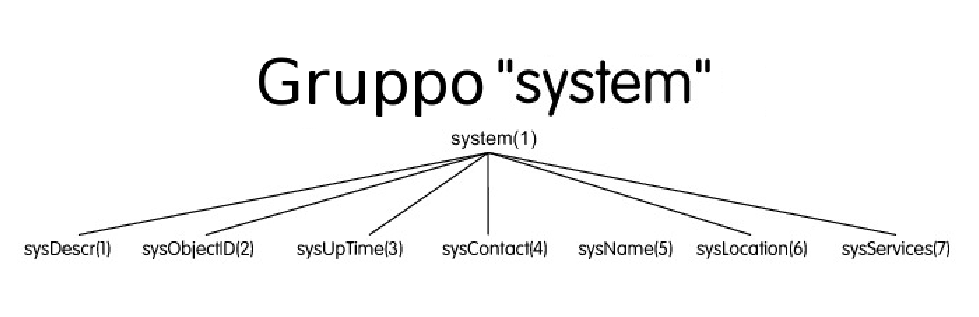
\includegraphics{figure/MIB_II_gruppo_system.eps}
  \caption{MIB II: gruppo ``system''}
\end{figure}

\begin{itemize}
\item La variabile {\tt sysUpTime.0} � veramente importante dato che serve a determinare le discontinuit� del servizio:
  \begin{itemize}
  \item se $sysUpTime.0_{t1} > sysUpTime.0_{t2}$ dove $t2 > t1$ allora l'agent � stato reinizializzato e le applicazioni di gestione si affidano a valori precedenti.
  \end{itemize}
\item {\tt sysService} riporta informazioni circa i servizi forniti dal sistema (si veda figura \ref{MIB_II_gruppo_syste_variabile_sysService}).
  \begin{figure}[htbp]
    \centering
    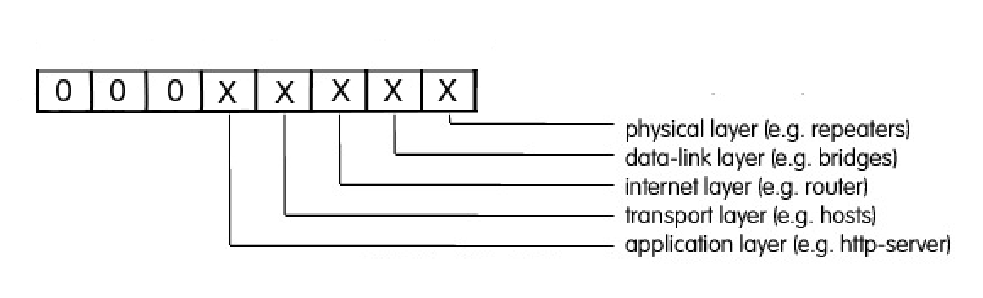
\includegraphics{figure/MIB_II_gruppo_system_variabile_sysService.eps}
    \caption{MIB II: gruppo ``system'', variabile sysService}
    \label{MIB_II_gruppo_syste_variabile_sysService}
  \end{figure}
\item {\tt sysObjectId.0} ha il formato {\tt enterprises.<prodotto>.<id>+} ed � usato per identificare il prodotto e il modello. Per esempio {\tt enterprises.9.1.208} identifica il Cisco (.9) 2600 router (.1.208).
\item {\tt sysDescr.0} fornisce una precisa descrizione del dispositivo (ad esempio ``Cisco Internetwork Operating System Software IOS (tm) C2600 Software (C2600-I-M), Version 12.2(23), RELEASE SOFTWARE (fc2) Copyright (c) 1986-2004 by cisco Systems, Inc.'').
\item In breve il gruppo ``system'' � importante per:
  \begin{itemize}
  \item Mappare i dispositivi (via {\tt sysObjectId.0}, {\tt sysDescr.0} e {\tt sysLocation.0}\footnote{Specifica dove si trova fisicamente il dispositivo}).
  \item Controllare il contatore del dispositivo ({\tt sysUpTime.0}).
  \item Riportare i problemi all'amministratore ({\tt sysContact.0}).
  \end{itemize}
\end{itemize}

\subsubsection{Gruppo ``interface''}

\begin{figure}[htbp]
  \centering
  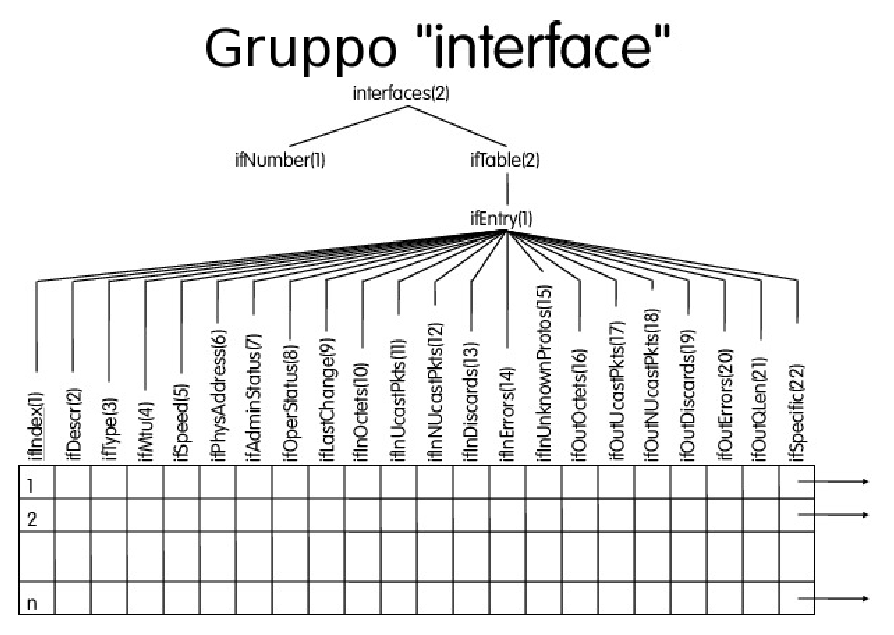
\includegraphics{figure/MIB_II_gruppo_interface.eps}
  \caption{MIB II: gruppo ``interface''}
\end{figure}

Informazioni sulle interfacce. Esiste una riga per ogni interfaccia ``attiva''. Se un'interfaccia viene ``spenta'' in un secondo momento, la sua riga rimane vuota (le righe successive non vengono spostate per chiudere il buco), quindi la variabile {\tt ifIndex} pu� presentare dei ``buchi''.
\begin{itemize}
\item {\tt sysAdminStatus}: il corrente stato amministrativo dell'interfaccia. Pu� essere: {\tt up(1)}, {\tt down(2)}, {\tt test(3)}. Un valore diverso da {\tt up} significa che l'interfaccia non � fisicamente presente oppure c'� ma non � disponibile al sistema operativo (ad esempio il driver non � stato caricato).
\item {\tt ifOperStatus}: il corrente stato operazionale dell'interfaccia. Pu� essere: {\tt up(1)}, {\tt down(2)}, {\tt test(3)}. Simile a {\tt ifconfig <device> up/down}.
\item {\tt ifOutQLen}: la lunghezza della coda dei pacchetti in uscita (misurata in pacchetti). \`E usata per conoscere qualcosa in pi� a proposito della velocit� di trasmissione e del throughput (se il buffer � pieno allora il destinatario non � veloce come il mittente).
\item {\tt ifLastChange}: contiene il valore del {\tt sysUpTime} al momento in cui l'interfaccia � entrata nello stato operazionale corrente. Usata per determinare quando un'interfaccia ha cambiato il suo stato operazionale (vedi {\tt ifOperStatus}).

  \begin{figure}[htbp]
    \centering
    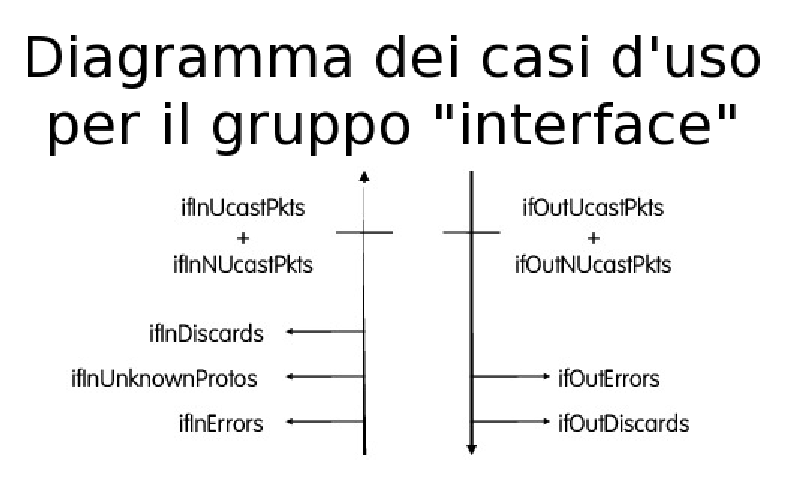
\includegraphics{figure/MIB_II_gruppo_interface_diagramma_dei_casi_d_uso.eps}
    \caption{MIB II: gruppo ``interface'': diagramma dei casi d'uso}
    \label{gruppo_interface_diagramma_dei_casi_d_uso}
  \end{figure}

  Il diagramma dei casi d'uso (figura \ref{gruppo_interface_diagramma_dei_casi_d_uso}) mostra le dipendenze tra le variabili:
  \begin{itemize}
  \item Il numero di pacchetti consegnati dall'interfaccia di rete al protocollo di livello superiore si calcola come:\\
    ${\tt ifInUcastPkts}\footnote{Il numero di pacchetti che non sono n� \glstext{multicast} n� \glstext{broadcast}.} + {\tt ifInNUcastPkts}\footnote{Il numero di pacchetti che sono o \glstext{multicast} o \glstext{broadcast}.}$
  \item Il numero di pacchetti ricevuti dalla rete si calcola come:\\
    $({\tt ifInUcastPkts} + {\tt ifInNUcastPkts}) + {\tt ifInDiscards}\footnote{Il numero di pacchetti scartati bench� non sono affetti da errore ed hanno un protocollo conosciuto (un esempio sono i pacchetti scartati per lasciare spazio nel buffer).} + {\tt ifInUnknownProtos}\footnote{Il numero di pacchetti scartati perch�, o non si conosce il protocollo, oppure non � gestito.} + {\tt ifInErrors}\footnote{Il numero di pacchetti scartati perch� affetti da errore.}$
  \end{itemize}
\end{itemize}

Uso del gruppo ``interface'':
\begin{itemize}
\item \`E la base del monitoraggio basato su SNMP.
\item Molti strumenti periodicamente prelevano i valori delle interfaccia (per lo pi� {\tt ifInOctets}\footnote{Il numero di ``ottetti'' (byte) ricevuti dall'interfaccia.}\\
  e {\tt ifOutOctets}\footnote{Il numero di ``ottetti'' (byte) inviati dall'interfaccia.}).
\item I valori sono aggregati e non divisi per protocollo di destinazione, \gls{AS}. Questa � la maggiore limitazione se si vuole fare un monitoraggio pi� mirato. La ragione � che i contatori SNMP sono semplicemente i contatori del kernel ``esposti'' via SNMP.
\item Errori delle interfacce possono essere usati per scovare dei problemi di comunicazione, specialmente con i link \gls{WAN}.
\item Le statistiche sulla dimensione dei pacchetti non vengono riportate, ma comunque si posso calcolare semplici statistiche usando il numero totale di ottetti e di pacchetti.
\item Molti produttori (ad esempio Cisco, Juniper) riportano delle informazioni a proposito sia delle interfacce fisiche che di quelle logiche (anche conosciute come sottointerfacce). Altri (ad esempio Extreme) hanno delle entry nella tabella ma i contatori sono sempre a zero.
\item Usando i contatori dell'interfaccia � possibile produrre un resoconto a proposito di:
  \begin{itemize}
  \item VLAN (Virtual LAN).
  \item PVC (Private Virtual Circuit) sui link Frame Relay\footnote{Il Frame Relay � una tecnica di trasmissione a commutazione di pacchetti (una tecnica di accesso multiplo a ripartizione nel tempo, usata per condividere un canale di comunicazione tra pi� stazioni in modo non deterministico).}.
  \end{itemize}
\end{itemize}

\subsection{Come calcolare la percentuale di utilizzo della larghezza di banda con SNMP}
$\%utilizzo\ della\ larghezza\ di\ banda = \frac{(\Delta ifInOctets + \Delta ifOutOctets)\times 8}{(\Delta tempo) \times IfSpeed} \times 100$
\bigskip
\\
$\%utilizzo\ in\ input = \frac{(\Delta ifInOctets) \times 8}{(\Delta tempo) \times IfSpeed} \times 100$
\bigskip
\\
$\%utilizzo\ in\ output = \frac{(\Delta ifOutOctets) \times 8}{(\Delta tempo) \times IfSpeed} \times 100$
\bigskip\\
Si noti che tutte le variabili necessarie si trovano nel gruppo {\tt interface}, mentre il $\Delta tempo$ viene ottenuto con la variabile {\tt sysUpTime.0}.
\subsubsection{Usare il gruppo ``arp''}
\begin{itemize}
\item Usato per accedere alla tabella \gls{ARP} dei dispositivi remoti.
\item Pu� essere usato per identificare gli attacchi di \glstext{ARP poisoning} oppure host mal configurati (ad esempio se ci sono indirizzi IP duplicati).
\item Esempio:
  {\footnotesize
\begin{verbatim}
    RFC1213-MIB::atIfIndex.4.1.172.22.6.168 = INTEGER: 4
    RFC1213-MIB::atIfIndex.4.1.172.22.7.255 = INTEGER: 4
    RFC1213-MIB::atPhysAddress.4.1.172.22.6.168 = Hex-STRING: 00 40 F4 67 49 08
    RFC1213-MIB::atPhysAddress.4.1.172.22.7.255 = Hex-STRING: FF FF FF FF FF FF
    RFC1213-MIB::atNetAddress.4.1.172.22.6.168 = Network Address: AC:16:06:A8
    RFC1213-MIB::atNetAddress.4.1.172.22.7.255 = Network Address: AC:16:07:FF
\end{verbatim}
  }
\end{itemize}

\subsection{Il MIB Bridge}
\begin{itemize}
\item Usato per controllare lo stato degli switch L2/L3. Non si commetta l'errore comune di credere che viene usato solo sui bridge\footnote{I bridge, gli switch e gli hub lavorano a livello 2 (Data Link) mentre a livello 3 (Network) troviamo i router. L'hub smista i pacchetti a tutte le interfacce con cui � collegato, un bridge o uno switch invece sanno indirizzare il pacchetto ad una specifica interfaccia. La differenza sostanziale tra un bridge e uno switch sta nel fatto che quest'ultimo ha molte pi� porte.}
\item \`E qualcosa di complementare al MIB II, dato che fornisce informazioni sugli host connessi alle porte dello switch.
\item Gli usi comuni del MIB bridge sono:
  \begin{itemize}
  \item Conoscere l'indirizzo MAC di un host connesso alla porta X/unit� Y dello switch\footnote{I grandi switch sono divisi per unit� poste una sopra l'altra, ogni unit� ha un insieme di porte.}\\
    {\tt dot1dTpFdbTable\footnote{\`E la tabella che contiene le informazioni a proposito degli host per i quali il bridge ha inviato o filtrato informazioni.}.dot1dTpFdbAddress\footnote{L'indirizzo MAC.}} (nota: il MIB II ha l'indirizzo MAC della porta dello switch).
  \item L'associazione porta/indirizzo MAC � la base per determinare dove si trova fisicamente un host. Infatti le porte dello switch sono generalmente connessehttp://42cows.org/ilfatto20101102.pdf alle prese della parete, e questo � un buon metodo per sapere chi c'� e dov'� ($utente \rightarrow computer \rightarrow porta\ dello\ switch \rightarrow stanza/scrivania$).
  \item Tiene traccia del ``precedente'' indirizzo MAC (e del tempo) connesso ad una porta, in questo modo � possibile tracciare gli utenti che si spostano da una stanza ad un altra.
  \item Pu� essere usato per trovare le porte che hanno pi� indirizzi MAC associati (un trunk) e quindi trovare gli utenti che hanno pi� indirizzi MAC (ad esempio gli utenti che hanno avviato una macchina virtuale come VMware, oppure gli utenti che hanno un virus/worm), oppure le porte che sono direttamente connesse ad un altro switch.
  \end{itemize}
\end{itemize}

\subsubsection{Esempio: prelevare indirizzi MAC e le porte fisiche}
\begin{enumerate}
\item Del bridge con indirizzo IP 14.32.6.17 si prelevano tutte le VLAN, vtpVlanState (.1.3.6.1.4.1.9.9.46.1.3.1.1.2 ):
{\footnotesize
\begin{verbatim}
# snmpwalk -c public 14.32.6.17 vtpVlanState
CISCO-VTP-MIB::vtpVlanState.1.1 = INTEGER: operational(1)
CISCO-VTP-MIB::vtpVlanState.1.2 = INTEGER: operational(1)
CISCO-VTP-MIB::vtpVlanState.1.6 = INTEGER: operational(1)
CISCO-VTP-MIB::vtpVlanState.1.7 = INTEGER: operational(1)
CISCO-VTP-MIB::vtpVlanState.1.8 = INTEGER: operational(1)
...
\end{verbatim}
}
\item Per ogni VLAN si prende la tabella degli indirizzi MAC (si noti la forma {\tt <read\_community>@<vlan\_number>}), dot1dTpFdbAddress (.1.3.6.1.2.1.17.4.3.1.1). Nell'esempio che segue, la VLAN 2 non ha niente nella sua tabella:
{\footnotesize
\begin{verbatim}
# snmpwalk -c public@1 14.32.6.17 dot1dTpFdbAddress
.1.3.6.1.2.1.17.4.3.1.1.0.208.211.106.71.251 = Hex-STRING: 00 D0 D3 6A 47 FB

# snmpwalk -c public@2 14.32.6.17 dot1dTpFdbAddress

# snmpwalk -c public@6 14.32.6.17 dot1dTpFdbAddress
.1.3.6.1.2.1.17.4.3.1.1.0.2.185.144.76.102 = Hex-STRING: 00 02 B9 90 4C 66
.1.3.6.1.2.1.17.4.3.1.1.0.2.253.106.170.243 = Hex-STRING: 00 02 FD 6A AA F3
.1.3.6.1.2.1.17.4.3.1.1.0.224.30.159.10.210 = Hex-STRING: 00 E0 1E 9F 0A D2

... e cos� via per tutte le VLAN scoperte al primo passaggio.
\end{verbatim}
}
\item Per ogni VLAN si preleva il numero di porta del bridge, dot1dTpFdbPort (.1.3.6.1.2.1.17.4.3.1.2):
{\footnotesize
\begin{verbatim}
# snmpwalk -c public@1 14.32.6.17 dot1dTpFdbPort
.1.3.6.1.2.1.17.4.3.1.2.0.208.211.106.71.251 = INTEGER: 113

# snmpwalk -c public@2 14.32.6.17 dot1dTpFdbPort

# snmpwalk -c public@6 14.32.6.17 dot1dTpFdbPort
.1.3.6.1.2.1.17.4.3.1.2.0.2.185.144.76.102 = INTEGER: 113
.1.3.6.1.2.1.17.4.3.1.2.0.2.253.106.170.243 = INTEGER: 113
.1.3.6.1.2.1.17.4.3.1.2.0.224.30.159.10.210 = INTEGER: 65

... e cos� via per tutte le VLAN scoperte al primo passaggio.
\end{verbatim}
}
\item Si prendono gli ifIndex delle porte del bridge, dot1dBasePortIfIndex (.1.3.6.1.2.1.17.1.4.1.2):
{\footnotesize
\begin{verbatim}
# snmpwalk -c public@1 14.32.6.17 dot1dBasePortIfIndex
.1.3.6.1.2.1.17.1.4.1.2.68 = INTEGER: 12
.1.3.6.1.2.1.17.1.4.1.2.69 = INTEGER: 13
.1.3.6.1.2.1.17.1.4.1.2.70 = INTEGER: 14
...
.1.3.6.1.2.1.17.1.4.1.2.113 = INTEGER: 57
...

... e cos� via per tutte le VLAN scoperte al primo passaggio.
\end{verbatim}
}
\item Quindi si attraversa ifName (.1.3.6.1.2.1.31.1.1.1.1) in modo che gli ifIndex ottenuti nel passaggio precedente possano essere associati al relativo nome della porta:
{\footnotesize
\begin{verbatim}
# snmpwalk -On -c public 14.32.6.17 ifName
.1.3.6.1.2.1.31.1.1.1.1.1 = STRING: sc0
.1.3.6.1.2.1.31.1.1.1.1.2 = STRING: sl0
.1.3.6.1.2.1.31.1.1.1.1.3 = STRING: me1
...
.1.3.6.1.2.1.31.1.1.1.1.57 = STRING: 2/49
...
\end{verbatim}
}
\end{enumerate}

Le informazioni raccolte possono essere usate, ad esempio:
\begin{enumerate}
\item Dal passo 2, c'� un indirizzo MAC:\\
  {\footnotesize {\tt .1.3.6.1.2.1.17.4.3.1.1.0.208.211.106.71.251 = Hex-STRING: 00 D0 D3 6A 47 FB}}
\item Il passo 3 ci dice che l'indirizzo MAC ({\tt 00 D0 D3 6A 47 FB}) si trova alla porta del bridge {\tt 113}:\\
  {\footnotesize {\tt .1.3.6.1.2.1.17.4.3.1.2.0.208.211.106.71.251 = INTEGER: 113}}
\item Dal passo 4, la porta {\tt 113} del bridge ha un ifIndex numero {\tt 57}:\\
  {\footnotesize {\tt .1.3.6.1.2.1.17.1.4.1.2.113 = INTEGER: 57}}
\item Dal passo 5, l'ifIndex {\tt 57} corrisponde alla porta fisica {\tt 2/49}:\\
  {\footnotesize {\tt .1.3.6.1.2.1.31.1.1.1.1.57 = STRING: 2/49}}
\end{enumerate}

\subsubsection{Note a margine: SNMP verso contatori \glsentrytext{CLI}}
\begin{itemize}
\item \`E una comune convinzione tra le community degli amministratori di rete pensare che SNMP e i contatori \gls{CLI} siano due modi diversi di vedere la stessa cosa\footnote{In questo contesto i contatori CLI sono dei contatori forniti dai device attraverso altre vie che non usano SNMP, ad esempio anche attraverso un'interfaccia HTML. La differenza sostanziale tra i contatori CLI e i contatori SNMP e che gli ultimi hanno il formato dell'output ben specifico, mentre i primi no, dipende da produttore a produttore.}.
\item Molti amministratori preferisco di pi� i contatori \gls{CLI} perch�:
  \begin{itemize}
  \item Hanno un formato direttamente consultabile dall'uomo
    \begin{itemize}
    \item 0 pacchetti in input, 0 pacchetti in output
    \end{itemize}
  \item Molte implementazioni forniscono comandi per cancellare/resettare i contatori
    \begin{itemize}
    \item clear interface ethernet 3
    \end{itemize}
  \end{itemize}
\item Nota: la definizione di cosa conta un contatore dipende dalla documentazione del prodotto.
\item
  {\footnotesize
\begin{verbatim}
c4500#sh int e1
Ethernet1 is up, line protocol is down
Last clearing of "show interface" counters never
Output queue 0/40, 0 drops; input queue 0/75, 0 drops
0 packets input, 0 bytes, 0 no buffer
     Received 0 broadcasts, 0 runts, 0 giants
     0 input errors, 0 CRC, 0 frame, 0 overrun, 0 ignored, 0 abort
     0 input packets with dribble condition detected
     187352 packets output, 11347294 bytes, 0 underruns
     187352 output errors, 0 collisions, 3 interface resets
\end{verbatim}
  }
\item Note:
  \begin{itemize}
  \item I contatori \gls{CLI} rimangono la via basilare per la gestione degli elementi.
  \item Il formato/apparenza dei contatori cambiano da produttore a produttore (spesso anche con lo stesso prodotto, ad esempio Cisco IOS verso CatOS verso PIX).
  \item Nota: IOS, CatOS e PIX sono rispettivamente router, switch e firewall OS usati dalle apparecchiature Cisco.
  \end{itemize}
\item I contatori SNMP invece:
  \begin{itemize}
  \item Offrono la possibilit� di confrontare le apparecchiature:
    \begin{itemize}
    \item Sono contatori definiti da uno standard
      \begin{itemize}
      \item Come definita da IETF\footnote{Internet Engineering Task Force}, IEEE\footnote{Institute of Electrical and Electronics Engineering}, qualche produttore, etc\ldots
      \item Non dipendono dai tipi di elementi di rete o dai produttori.
      \end{itemize}
    \item Sono unici a livello globale, con nomi difficili da pronunciare
      \begin{itemize}
      \item {\tt 1.3.6.1.2.1.17.2.4 dot1dStpTopChanges}
      \end{itemize}
    \end{itemize}
  \item Hanno una dimensione ben specifica
    \begin{itemize}
    \item Larghezza a 32 o a 64 bit (i 64 bit sono disponibili in SNMP v2c o v3).
    \end{itemize}
  \item I contatori non necessariamente partono da zero
    \begin{itemize}
    \item I produttori sono liberi di fare quello che vogliono.
    \end{itemize}
  \item Non sono pensati per essere consultati direttamente dall'uomo.
  \item
    {\footnotesize
\begin{verbatim}
dot1dTpPortInFrames OBJECT-TYPE
              SYNTAX Counter
              ACCESS read-only
              STATUS mandatory
              DESCRIPTION
                    "The number of frames that have been received by
                    this port from its segment. Note that a frame
                    received on the interface corresponding to this
                    port is only counted by this object if and only if
                    it is for a protocol being processed by the local
                    bridging function, including bridge management
                    frames."
              REFERENCE
                    "IEEE 802.1D-1990: Section 6.6.1.1.3"
\end{verbatim}
    }
  \item Nota: i buoni contatori generalmente derivano da una specificazione del protocollo sottostante.
  \end{itemize}
\end{itemize}

\subsection{Cos'altro si pu� fare con SNMP?}
\begin{itemize}
\item Individuare ed eliminare le connessioni TCP pendenti.
\item Manipolare la tabella \gls{ARP}.
\item Prelevare la temperatura ambientale.
\item Controllare l'utilizzo della CPU.
\item Monitorare gli alimentatori e/o i gruppi di continuit�.
\item Trovare gli utenti che usano \gls{P2P} (utilizzando la tabella NAT\footnote{Network Address Translation.}).
\item Visualizzare la topologia della rete (ad esempio con CDP\footnote{Cisco Discovery Protocol.}).
\end{itemize}

% LocalWords:  SNMP MIB RFC ICMP UDP TCP stack routing l'IP IPv system' l'agent
% LocalWords:  sysUpTime sysService sysObjectId Cisco router sysDescr Operating
% LocalWords:  Internetwork System IOS tm Version fc cisco Systems Inc spenta'
% LocalWords:  sysLocation sysContact interface' ifIndex buchi' sysAdminStatus
% LocalWords:  ifOperStatus ifconfig device ifOutQLen throughput ifLastChange
% LocalWords:  ifInUcastPkts multicast broadcast ifInNUcastPkts ifInDiscards AS
% LocalWords:  ifInUnknownProtos ifInErrors ifInOctets ottetti' ifOutOctets WAN
% LocalWords:  esposti' Wide Juniper sottointerfacce Extreme entry VLAN Virtual
% LocalWords:  PVC Circuit Relay IfSpeed interface arp' ARP Address Resolution
% LocalWords:  Protocol arp poisoning L'ARP spoofing attacker switched lan the
% LocalWords:  middle cache host switch hub L'hub MAC unit dot dTpFdbTable worm
% LocalWords:  dTpFdbAddress precedente' trunk VMware vtpVlanState read number
% LocalWords:  dTpFdbPort dBasePortIfIndex ifName Hex STRING FB INTEGER Command
% LocalWords:  l'ifIndex Line community clear ethernet CatOS PIX firewall OS of
% LocalWords:  IETF Force IEEE Institute Electrical and Electronics NAT CDP
% LocalWords:  dStpTopChanges Translation Discovery

\section{Monitoraggio remoto}

\subsection{Le reti stanno cambiando}
\begin{tabular}{p{.28\textwidth}p{.333\textwidth}p{.313\textwidth}}
  Internet:
  \begin{itemize}
  \item La sicurezza di rete inizier� ad essere un elemento pi� critico nel futuro.
  \item Le reti aziendali diventeranno reti pubbliche.
  \end{itemize}
  &
  Telefonia:
  \begin{itemize}
  \item Il supporto alla telefonia attraverso reti wired e wireless saranno un elemento chiave delle reti future.
  \item La rete diventer� sempre e dovunque una risorsa.
  \end{itemize}
  &
  Comunicazioni dinamiche:
  \begin{itemize}
  \item Il supporto ad un ampio numero di applicazioni sar� l'elemento chiave del futuro: convergenza.
  \item I dati della rete saranno la rete.
  \end{itemize}
\end{tabular}

\begin{figure}[htbp]
  \centering
  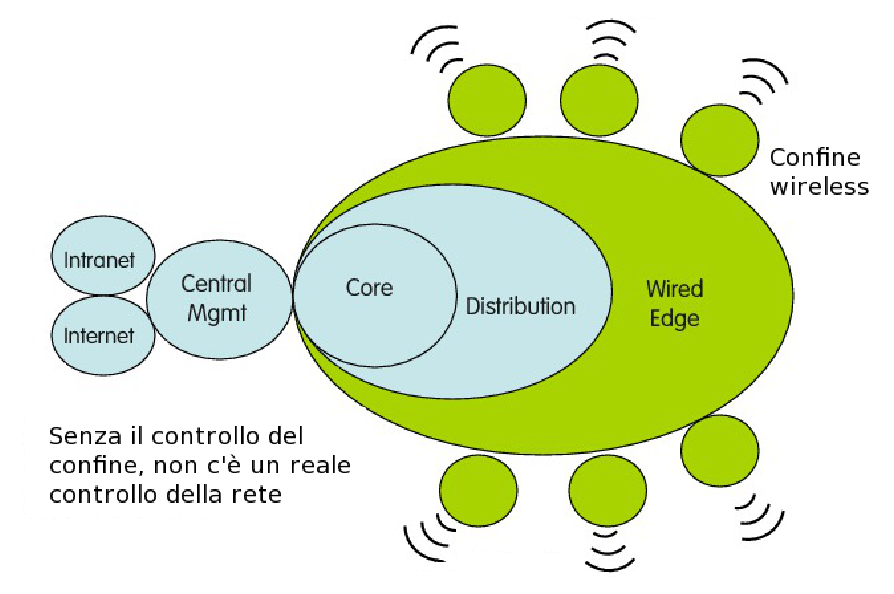
\includegraphics{figure/La_rete_sta_cambiando.eps}
  \caption{La rete sta cambiando}
\end{figure}

\subsection{Verso il monitoraggio remoto}
\begin{itemize}
\item Le reti moderne sono distribuite tra varie costruzioni, amministrate da persone differenti con varie competenze (sicurezza, analizzatore di traffico, amministratore di database).
\item \`E necessario raccogliere le statistiche del traffico su ogni tronco della rete e spedirle ad un (limitato) numero di collezionatori, in modo da produrre una vista globale.
\item Qualche capacit� di analisi distribuita � necessaria perch� una rete centralizzata non � scalabile e non supporta gli errori.
\item Sistemare gli analizzatori di traffico (ad esempio sonde basate su pcap) non � sempre fattibile perch�:
  \begin{itemize}
  \item I server non sempre permettono l'installazione di generici software non testati (ad esempio, la licenza pu� obbligare di installare su di un server Oracle solo applicazioni certificate da Oracle).
  \item I server moderni hanno spesso molte interfacce di rete (1 Gb principale pi� failover per i dati e 100 Mbit per l'accesso al server). Su questi server � necessario installare delle sonde multi-interfacce.
  \item Monitorare una 1 GE richiede 2xGE (una per ogni RX\footnote{Comunicazione in entrata (receive).} dell'originale GE).
  \end{itemize}
\item Soluzione: usare le capacit� di analisi del traffico delle apparecchiature di rete.
\item Svantaggi:
  \begin{itemize}
  \item Non tutte le apparecchiature sono fornite di capacit� di analisi del traffico (ad esempio molti router ADSL non le hanno).
  \item Anche se supportate, non sempre queste capacit� possono essere abilitate (forte impatto sulla CPU e la memoria).
  \item Le capacit� di monitoraggio base fornite dai sistemi operativi di default sono piuttosto limitate e quindi � necessario una scheda personalizzata.
  \item Le schede personalizzate per l'analisi del traffico non sono economiche.
  \end{itemize}
\item Ecco i prezzi di qualche scheda di monitoraggio in commercio (il software va comprato a parte):\\
  \begin{tabular}{|c|c|}
    \hline
    Prodotto & Prezzo (solo scheda)\\
    \hline
    Cisco MSFC-2 & 46'000 \$\\
    \hline
    Juniper PM-PIC & 30'000 \$\\
    \hline
  \end{tabular}
\end{itemize}

\subsection{RMON: Monitoraggio remoto usando SNMP}
\begin{itemize}
\item Presente su molte medio/alte apparecchiature di rete: spesso queste sono povere/limitate implementazioni.
\item Qualche produttore vende delle sonde stand-alone. Quelle preferite sono quelle che:
  \begin{itemize}
  \item sono piene implementazioni del protocollo.
  \item non aggiungono altro carico al router.
  \end{itemize}
\item Esistono due versioni di RMON, RMON1 (RMON v1) e RMON2 (RMON v2). Mentre RMON1 � specializzato solo per i primi 2 livelli della pila ISO/OSI, RMON2 si concentra sui livelli dal 3 al 6.
\item Non tutte le implementazioni (in particolare quelle embedded nei router/switch) supportano l'intero standard ma solo alcuni selezionati gruppi SNMP.
\item Insieme con Cisco NetFlow � l'industriale, ``fidato'', standard di monitoraggio.
\end{itemize}

\subsubsection{Cosa pu� fare RMON}
\begin{itemize}
\item Raccogliere dati e periodicamente inviarli a dei centri di gestione, i quali potenzialmente riducono il traffico sui link \gls{WAN} e spostano l'overhead sui centri di gestione.
\item Riportano ci� che fanno gli host della rete, quanto ``parlano'', e verso chi.
\item ``Vedere'' tutto il traffico \gls{LAN}, l'utilizzo della \gls{LAN}, e non solo il traffico verso o attraverso il router.
\item Filtra e cattura i pacchetti (quindi non c'� bisogno di controllare o  inserire un analizzatore \gls{LAN}): � in pratica uno sniffer remoto che pu� catturare il traffico in real-time (finch� non finisce la memoria integrata).
\item Automaticamente raccoglie i dati, confronta le soglie, e spedisce segnali al centro di gestione - il quale scarica molto del lavoro che potrebbe impantanare il centro di gestione.
\end{itemize}

\subsubsection{RMON verso SNMP}
\begin{itemize}
\item Il protocollo SNMP viene usato per configurare e controllare una sonda. Generalmente la gestione con le interfacce grafiche utente (GUI - Graphic User Interface) nasconde la complessit� della configurazione basata su SNMP.
\item Usando SNMP le applicazioni di amministrazione possono ricevere le statistiche e il traffico salvato in modo da registrare le statistiche di una rete con la possibilit� di selezionarne una parte.
\item SNMP e RMON differiscono nel modo in cui raccolgono le statistiche sul traffico:
  \begin{itemize}
  \item Con SNMP vengono fatte delle richieste periodiche: richiede una query al dispositivo SNMP per prendere le statistiche di rete (lo stato della rete viene preso dal manager).
  \item RMON, in modo diverso, riduce il lavoro del manager raccogliendo e salvando le statistiche in contatori o buckets pronte per essere ricevute da un centro di amministrazione.
  \end{itemize}
\end{itemize}

\subsubsection{RMON1 filtri e canali}
\begin{itemize}
\item I pacchetti ricevuti possono essere filtrati. I filtri sono semplici espressioni di valori/maschere (come indirizzo IP, rete e maschera).
\item Un canale RMON � definito come un'insieme di coppie di filtri: uno sui dati (sul pacchetto) e uno sullo stato (sulle informazioni del pacchetto, come ad esempio la dimensione).
\item Un pacchetto viene accettato da un canale quando:
  \begin{itemize}
  \item ha una corrispondenza con almeno una coppia di filtri ({\tt acceptMatched channel}).
  \item almeno un filtro di tutte le coppie di filtri fallisce il test ({\tt acceptFailed channel}).
  \end{itemize}
\end{itemize}

\begin{figure}[htbp]
  \centering
  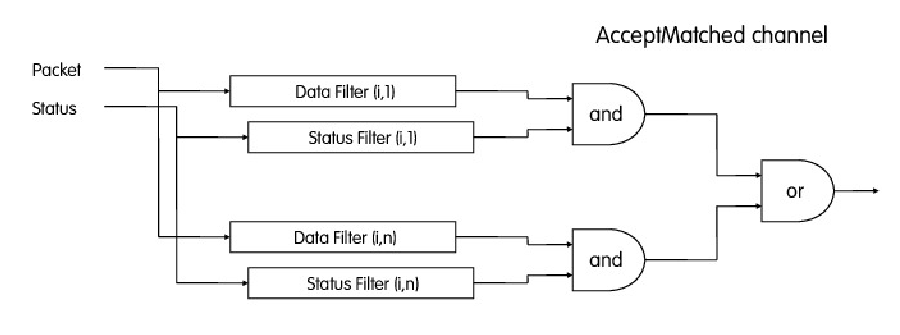
\includegraphics{figure/RMON_1_filtri_canali.eps}
  \caption{RMON: {\tt acceptMatched channel}. Nell'{\tt acceptFailed channel}, le porte AND diventano OR e la porta OR diventa AND.}
\end{figure}

\subsubsection{I gruppi di monitoraggio RMON1}
\begin{tabular}{|p{0.1214\textwidth}|p{0.377\textwidth}|p{0.43\textwidth}|}
  \hline
  Gruppi & Funzioni & Elementi\\
  \hline
  Statistics & Contiene le statistiche misurate dalla sonda per ogni interfaccia monitorata su questo dispositivo. & Pacchetti scartati, pacchetti spediti, byte spediti (``ottetti''), pacchetti di \glstext{broadcast}, pacchetti \glstext{multicast}.\\
  \hline
  History & Registra alcune statistiche campione dalla rete e le salva per essere prelevate pi� tardi. & Periodo campione, numero di campioni, i campioni.\\
  \hline
  Alarm & Periodicamente preleva dei campioni statistici dalla sonda e li confronta con delle soglie configurate precedentemente. Se la variabile monitorata supera una soglia, allora si genera un evento. & Tipo di allarme, soglia inferiore, soglia superiore.\\
  \hline
  Host & Contiene le statistiche associate ad ogni host scoperto in rete. & Indirizzo dell'host e byte ricevuti e trasmessi sia su \glstext{broadcast} che su \glstext{multicast} e pacchetti errati.\\
  \hline
  HostTopN & Prepara tabelle che descrivono i top-host (quelli che usano di pi� la rete) in una lista ordinata per un tipo di statistica sull'intervallo specificato dal centro di gestione. Perci� queste statistiche sono dipendenti dalla velocit�. & Statistiche, host, inizio e fine del periodo campione, velocit� di base, durata.\\
  \hline
  Matrix & Salva le statistiche sulle conversazioni tra due indirizzi settati. Come il dispositivo determina una nuova conversazione, crea una nuova entry nella tabella. & Tipo di filtro per i bit (maschera o non maschera), espressione del filtro (livello di bit), espressione condizionale (and, or, not) verso gli altri filtri.\\
  \hline
  Filters & Abilita dei filtri sui pacchetti. I pacchetti che passano il filtro formano un flusso di dati che pu� essere catturato oppure che pu� generare eventi. & Tipo di filtro per i bit (maschera o non maschera), espressione del filtro (livello di bit), espressione condizionale (and, or, not) verso gli altri filtri.\\
  \hline
  Packet Capture & Abilita la cattura dei pacchetti dopo che sono passati da un canale. & Dimensione del buffer per la cattura dei pacchetti, intero stato (allarme), numero dei pacchetti catturati.\\
  \hline
  Events & Controlla la generazione e la notifica degli eventi del dispositivo. & Tipo di evento, descrizione, il tempo di ultimo invio dell'evento.\\
  \hline
\end{tabular}

\subsubsection{Il gruppo ``alarm'' di RMON1}
\begin{figure}[htbp]
  \centering
  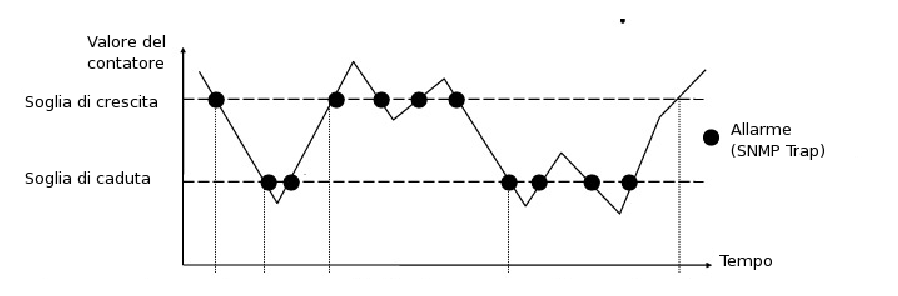
\includegraphics{figure/RMON_allarmi.eps}
  \caption{RMON: allarmi}
\end{figure}

\begin{itemize}
\item Un evento viene generato ogni volta che viene superata una soglia (o superiore o inferiore) o quando un valore sopra (o sotto) la soglia ritorna nei limiti.
\item Le soglie possono essere misurate o con un valore specifico (assoluto) oppure come differenza tra il valore attuale e l'ultimo valore misurato (valore delta).
\end{itemize}

\subsubsection{Statistiche ethernet di RMON}
\begin{description}
\item[Pacchetti:] un unit� di dati formattati per la trasmissione sulla rete.
\item [Pacchetti \glstext{multicast}:] comunicazione tra un singolo mittente e pi� destinatari nella rete.
\item [Pacchetti \glstext{broadcast}:] un pacchetto trasmesso a tutti gli host della ethernet.
\item [Eventi di scarto:] un superamento del limite della porta. La porta logica non � in grado di ricevere i pacchetti alla piena velocit� della linea e quindi inizia a scartarne qualcuno.
\item [Frammenti:] un pezzo di un pacchetto. Qualche volta un pacchetto di comunicazione che viene spedito in rete deve essere spezzato temporaneamente in frammenti; il pacchetto dovrebbe essere riassemblato quando raggiunge la destinazione.
\item [Jabber:] pacchetti ricevuti di dimensione maggiore a 1518 ottetti e che contengono anche errori di allineamento.
\item [Pacchetti sovradimensionati:] pacchetti di dimensione maggiore a 1518 ottetti ma che sono ben formati.
\end{description}

\subsubsection{Utilizzo della rete con RMON}
\begin{itemize}
\item Molti amministratori usano i contatori di RMON per calcolare l'utilizzo della rete.
\item L'utilizzo della rete pu� essere calcolata per tutte le porte dello switch ad intervalli regolari. Queste informazioni possono essere raccolte durante l'arco della giornata per poi generare un profilo dell'utilizzo dello switch o dell'hub.
\end{itemize}

$\%utilizzo\ della\ rete = \frac{(\#pacchetti \times 160) + (\#ottetti \times 8)}{(velocit\grave{a}\ della\ porta) \times (secondi)} \times 100$

\subsubsection{Caso di studio: intervallo di campionamento del contatore}

Esempio 1: (intervallo di campionamento di 10 secondi, valore di soglia 20, intervallo di test di 10 secondi)

\begin{tabbing}
  Soglia attuale da controllare: \= 0000 \= 0000 \= 0000\kill
  Tempo: \> 0 \> 10 \> 20\\
  Valore: \> 0 \> 19 \> 32\\
  Delta: \> \> 19 \> 13\\
  Soglia attuale da controllare: \> \> 19 \> 13
\end{tabbing}
\bigskip
Esempio 2: (intervallo di campionamento di 5 secondi, valore di soglia 20, intervallo di test di 10 secondi)
\begin{tabbing}
  Soglia attuale da controllare: \= 0000 \= 0000 \= 0000 \= 0000 \= 0000\kill
  Tempo: \> 0 \> 5 \> 10 \> 15 \> 20\\
  Valore: \> 0 \> 10 \> 19 \> 30 \> 32\\
  Delta: \> \> 10 \> 9 \> 11 \> 2\\
\end{tabbing}

\begin{itemize}
\item Il valore campione istanziato dal MIB deve essere fatto due volte per ogni intervallo di campionamento, altrimenti il superamento della soglia potrebbe non essere rilevato quando gli intervalli si sovrappongono.
\item Prelevare i valori velocemente (fast polling) ha questi svantaggi:
  \begin{itemize}
  \item Vengono collezionati molti dati.
  \item Si incrementa il carico dell'agent SNMP.
  \item Vengono rilevati molti cambiamenti (questo pu� portare a dei falsi positivi).
  \end{itemize}
\item Prelevare i valori lentamente (slow polling) ha questi svantaggi:
  \begin{itemize}
  \item Qualche allarme pu� essere perso (inesattezza).
  \end{itemize}
\end{itemize}

\subsection{Sonde migliorate in stile RMON}
\begin{itemize}
\item Ogni router/switch (spaziando da quelli Cisco a quelli basati su Linux) hanno la capacit� di definire delle liste di accesso controllato (ACL - Access Control List) per evitare in maniera preventiva un selezionato flusso di traffico.
\item Le ACL con la politica di ``accesso'' possono essere usate molto bene per controllare il traffico.
\item Svantaggi:
  \begin{itemize}
  \item Le ACL sono limitate agli IP laddove RMON no (ad esempio IPX, NeBEUI).
  \item Su molti sistemi, le ACL impattano sulla CPU.
  \item Il numero totale di ACL, per porta, � limitato.
  \item Spesso le ACL si limitano a controllare l'header del pacchetto (non il carico utile, il payload).
  \end{itemize}
\end{itemize}

Esempi di definizione delle ACL:
\begin{itemize}
\item Cisco\\
  {\footnotesize {\tt access-list 102 permit icmp any any}}
\item Juniper
  {\footnotesize
\begin{verbatim}
    filter HTTPcounter {
      from {
        destination-address {
          10.10.20/24;
          10.40.30/25;
          11.11/8;
        }
        destination-port [http https];
      }
      then {
        count Count-Http;
        accept
\end{verbatim}
  }
\item Linux (iptables)
  {\footnotesize
\begin{verbatim}
# /sbin/iptables -xnvL
Chain INPUT (policy ACCEPT 0 packets, 0 bytes)
   pkts       bytes                target   prot opt  in   out       source        destination
 236675   169960206   RH-Firewall-1-INPUT    all  --   *     *    0.0.0.0/0          0.0.0.0/0

Chain FORWARD (policy ACCEPT 0 packets, 0 bytes)
   pkts       bytes                target   prot opt  in   out       source        destination
      0           0   RH-Firewall-1-INPUT    all  --   *     *    0.0.0.0/0          0.0.0.0/0

Chain OUTPUT (policy ACCEPT 262868 packets, 233122676 bytes)
   pkts       bytes                target   prot opt  in   out       source        destination

Chain RH-Firewall-1-INPUT (2 references)
   pkts       bytes                target   prot opt  in   out       source        destination
  68169    81214627                ACCEPT    all  --  lo     *    0.0.0.0/0          0.0.0.0/0
    677       53751                ACCEPT   icmp  --   *     *    0.0.0.0/0          0.0.0.0/0
      0           0                ACCEPT    esp  --   *     *    0.0.0.0/0          0.0.0.0/0
      0           0                ACCEPT     ah  --   *     *    0.0.0.0/0          0.0.0.0/0
\end{verbatim}
  }
\end{itemize}

\begin{itemize}
\item I contatori sono in genere accessibili via SNMP con l'aiuto di un'interfaccia a riga di comando (\gls{CLI}).
\item I MIB proprietari abilitano la lettura dei valori anche in remoto.
\item La Cisco ha recentemente introdotto una nuova tecnologia chiamata ``Static NetFlow'' che abilita i router ad emettere i flussi per ogni ACL definita.
\item Il ``ClearFlow'' della Extreme Network � una tecnologia simile, ma con inoltre la capacit� di lanciare degli allarmi settando delle soglie sui valori dei contatori.
\end{itemize}

\subsection{NBAR: statistiche sul traffico in stile RMON}
\begin{itemize}
\item Cisco NBAR (Network Based Application Recognition) � un motore per la classificazione del traffico con il supporto a \gls{QoS} (cio� possono modellare il traffico in base alle statistiche).
\item Esegue l'analisi dei modelli di traffico in real-time (con l'analisi del payload) e scopre i protocolli.
\item Esempio di NBAR: fermare il traffico KaZaA e dare priorit� al traffico di video conferenza.
\item Ha la capacit� di classificare le applicazioni che hanno:
  \begin{itemize}
  \item I numeri di porta UDP o TCP staticamente assegnati.
  \item Protocolli che non sono TCP o UDP IP.
  \item Numeri di porta UDP o TCP assegnati dinamicamente durante la connessione.
  \item Classificazione basata su una ispezione profonda del pacchetto: NBAR pu� guardare all'interno di un pacchetto per identificare le applicazioni.
  \item Traffico HTTP via URL, nome dell'host o tipo MIME usando le espressioni regolari (*, ?, [ ]), Citrix ICA traffic, classificazione in base al tipo di payload RTP.
  \item Attualmente supporta 88 protocolli/applicazioni.
  \end{itemize}
\item Le statistiche di NBAR possono essere lette usando SNMP (Cisco NBAR Protocol Discovery MIB).
\item Attenzione:
  \begin{itemize}
  \item Tecnologia proprietaria: disponibile solo sulle apparecchiature Cisco con una recente versione di IOS\footnote{Il software Cisco IOS � la piattaforma che consente l'implementazione dei servizi di rete e abilita le applicazioni di networking basate su infrastrutture Cisco Systems.}
  \item Forte impatto sulla CPU dei router (pi� di NetFlow).
  \item Non riconosce tutti i protocolli.
  \item Difficile da configurare, in particolare se associato con l'amministrazione di \gls{QoS}/Larghezza di banda.
  \end{itemize}
\end{itemize}

{\footnotesize
\begin{verbatim}
Router# conf t
Router(config)# ip cef
Router(config)# int eth0/0
Router(config-if)# ip nbar protocol-discovery
Router(config-if)# exit
Router(config)# int se0/0
Router(config-if)# ip nbar protocol-discovery

Router# show ip nbar protocol discovery int eth0/0 top 3

FastEthernet0/0
Input                    Output
Protocol                 Packet Count             Packet Count
Byte Count               Byte Count
5 minute bit rate (bps)  5 minute bit rate (bps)
------------------------ ------------------------ ------------------------
ftp                      64175242                 45153848
89351513113              2484576000
1073000                  28000
http                     58194017                 32519125
82356099996              1958417833

Router# show policy-map int eth0/0

Ethernet0/0
Service-policy input: dscp_mark

Class-map: stream (match-any)
130521 packets, 97066868 bytes
5 minute offered rate 0 bps, drop rate 0 bps
Match: protocol rtp
0 packets, 0 bytes
5 minute rate 0 bps
Match: protocol rtspplayer
117857 packets, 79344153 bytes
5 minute rate 0 bps
Match: protocol netshow
12664 packets, 17722715 bytes
5 minute rate 0 bps
Match: ip dscp ef
0 packets, 0 bytes
5 minute rate 0 bps
QoS Set
\end{verbatim}
}

\begin{figure}[htbp]
  \centering
  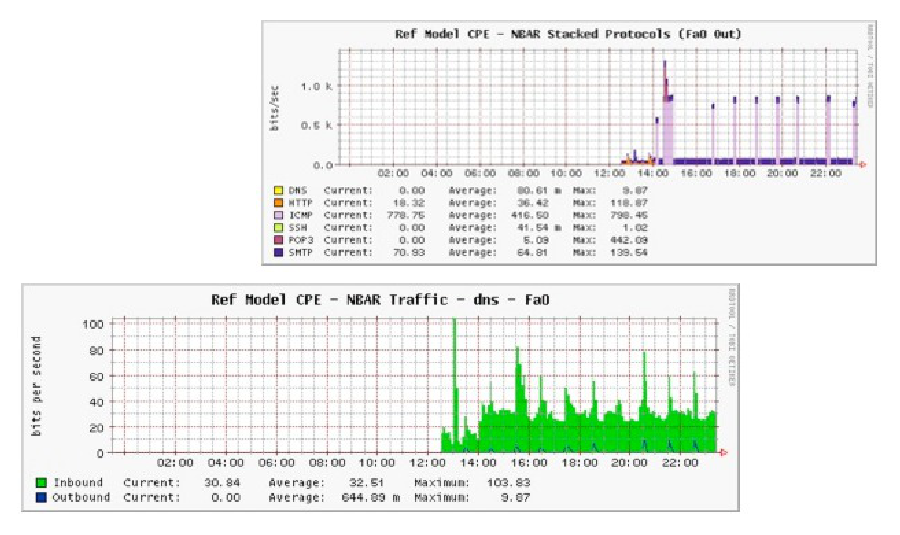
\includegraphics{figure/NBAR.eps}
  \caption{NBAR}
\end{figure}

\bigskip

\subsection{Misurazioni del flusso in real-time (RTFM - Real-Time Flow Measurement)}
\begin{minipage}{0.7\textwidth}
  \begin{itemize}
  \item Un ``Meter'' veramente flessibile e potente.
    \begin{itemize}
    \item Insiemi di regole programmabili.
    \item Pu� servire molti utenti.
    \item Si pu� programmare il comportamento al sovraccarico.
    \end{itemize}
  \item Il ``Reader'' pu� prendere i sondaggi.
  \item Realizzato sul MIB SNMP Meter.
  \item Esiste un'implementazione free software NeTraMet.
  \item I produttori non lo accettano volentieri, sebbene sia standard.
  \item Complicato da usare (troppo potente).
  \item Specificato dalle RFC 2720-2742.
  \end{itemize}
\end{minipage}%
\begin{minipage}[r]{0.3\textwidth}
  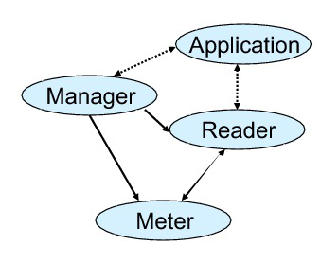
\includegraphics{figure/RTFM.eps}
\end{minipage}

% LocalWords:  wired wireless collezionatori pcap Oracle Gb failover Mbit GE RX
% LocalWords:  xGE receive router Cisco MSFC Juniper PM PIC RMON SNMP embedded
% LocalWords:  switch NetFlow l'overhead host parlano' sniffer GUI Graphic WAN
% LocalWords:  Interface query buckets acceptMatched channel acceptFailed Alarm
% LocalWords:  Statistics ottetti' broadcast multicast History dell'host Matrix
% LocalWords:  HostTopN entry and not Filters Packet Capture Events alarm'
% LocalWords:  ethernet
% LocalWords:  riassemblato Jabber dell'hub velocit istanziato MIB polling List
% LocalWords:  dell'agent Access Control IPX NeBEUI l'header payload access any
% LocalWords:  list permit icmp iptables Command Line Static ClearFlow' Extreme
% LocalWords:  NBAR Based Application Recognition QoS KaZaA UDP TCP URL MIME
% LocalWords:  Citrix ICA traffic RTP Protocol IOS networking Systems RTFM Flow
% LocalWords:  Measurement Reader' NeTraMet RFC

\section{Monitoraggio del flusso}
\subsection{I flussi}
\begin{itemize}
\item SNMP � basato su un paradigma manager-agent.
  \begin{itemize}
  \item L'agent monitora la rete ed informa il manager (via trap) quando qualcosa di importante � successo (ad esempio, un interfaccia ha cambiato stato).
  \item Il manager preleva l'intero stato del sistema periodicamente leggendo (polling) le variabili (ad esempio con le SNMP Get) dall'agent.
  \item Le variabili SNMP possono essere usate sia per la gestione di elementi/dispositivi/sistema (ad esempio sullo spazio del disco e sulle partizioni) che il monitoraggio del traffico.
  \end{itemize}
\item I flussi di rete invece sono emessi da una sonda verso uno o pi� collezionatori a seconda delle condizioni di traffico.
  \begin{itemize}
  \item I flussi contengono informazioni a proposito dell'analisi del traffico (cio� non contengono informazioni a proposito del dispositivo/sonda come con le variabili del MIB II).
  \item I flussi emessi hanno un formato ben definito (ad esempio Cisco NetFlow v5) e spesso usano UDP come livello di trasporto (non protocolli specializzati come SNMP).
  \item Non esiste il concetto di ``allarme'' sui flussi e la sonda non ha la capacit� di eseguire delle operazioni in base al traffico: tutta la parte intelligente sta nel collezionatore.
  \item L'instrumentazione della sonda viene fatta offline.
  \item Le sonde vengono attivate dove fluisce il traffico di rete (ad esempio nei router o negli switch).
  \end{itemize}
\end{itemize}

\subsubsection{Quindi, cosa ci si aspetta di misurare con i flussi}
\begin{itemize}
\item Con chi vi � uno scambio di traffico a seconda degli indirizzi IP, prefissi IP, o \gls{ASN}.
\item Quanto traffico e di che tipo (SMTP, WEB, file sharing, etc\ldots).
\item Che servizi girano ad esempio in un ateneo universitario.
\item Sommario dei traffici dei dipartimenti universitari.
\item Tracciare la sorgente degli attacchi \gls{DoS}, ad esempio i 100 server che hanno inondato il dominio XXX.com.
\item Trovare gli host che usano molto la rete (top host).
\item Con quante destinazioni ogni host ha del traffico.
\item Contare gli host che hanno dei servizi attivi, ad esempio quanti sono i server web attivi.
\end{itemize}

\subsubsection{Cosa non si pu� misurare con i flussi}
\begin{itemize}
\item Il traffico Non-IP (ad esempio NetBIOS, AppleTalk).
\item Le informazioni a livello 2 (ad esempio il cambiamento di stato down/up delle interfacce).
\item Il traffico filtrato (contare le politiche di un firewall).
\item Statistiche per link (ad esempio l'uso del link, congestione, il ritardo, i pacchetti persi).
\item Statistiche sulle applicazioni (ad esempio la latenza delle transazioni, il numero di risposte positive/negative, errori di protocollo).
\end{itemize}

\subsubsection{I flussi di rete: cosa sono?}
Un flusso � un insieme di pacchetti legati da un insieme comune di propriet� (ad esempio hanno stesso indirizzo IP e la stessa porta).

\subsubsection{Emissione dei flussi}
Un flusso viene (accodato) emesso solo quando lo si considera terminato.
\begin{itemize}
\item Politica di creazione e terminazione:
  \begin{itemize}
  \item Quali condizioni fanno iniziare e finire un flusso?
  \item Massima durata di un flusso senza considerare lo stato della connessione (ad esempio una connessione TCP finisce quando entrambi gli host si sono messi d'accordo sul FIN/RST).
  \item Emettere un flusso quando non c'� traffico per una certa quantit� di tempo.
  \end{itemize}
\end{itemize}

\subsubsection{I contenuti dei flussi di rete}
\begin{itemize}
\item Un flusso contiene:
  \begin{itemize}
  \item Host: sorgente e destinazione
  \item Contatori: pacchetti, byte, tempo.
  \item Informazioni sul routing: \gls{AS}, maschera di rete, interfacce.
  \end{itemize}
\item I flussi possono essere unidirezionali (di default) o bidirezionali (solo NetFlow v9 e IPFIX\footnote{Internet Protocol Flow Information Export (IPFIX) � la versione standardizzata dalla IETF del NetFlow v9 della Cisco.}).
\item Due opposti flussi unidirezionali corrispondono ad un unico flusso bidirezionale.
\item I flussi bidirezionali possono contenere altre informazioni coma il round trip time o il comportamento del TCP.
\end{itemize}

\subsubsection{I problemi dei flussi di rete}
\begin{itemize}
\item Overhead (carico della CPU) contro accuratezza:
  \begin{itemize}
  \item Molte misurazioni risultano in pi� dati collezionati.
  \item Molta aggregazione, meno granularit�.
  \item Overhead sui router, switch e host.
  \end{itemize}
\item Sicurezza contro condivisione dati:
  \begin{itemize}
  \item Il flusso emesso deve raggiungere il collezionatore attraverso un percorso protetto (ad esempio usando una differente rete/VLAN).
  \item La privacy dell'utente deve essere rispettata.
  \item Le misurazioni devono essere protette in modo da non divulgare informazioni importanti sulla rete a terze parti.
  \end{itemize}
\end{itemize}

\subsubsection{Esempi di flussi}
\begin{figure}[htbp]
  \centering
  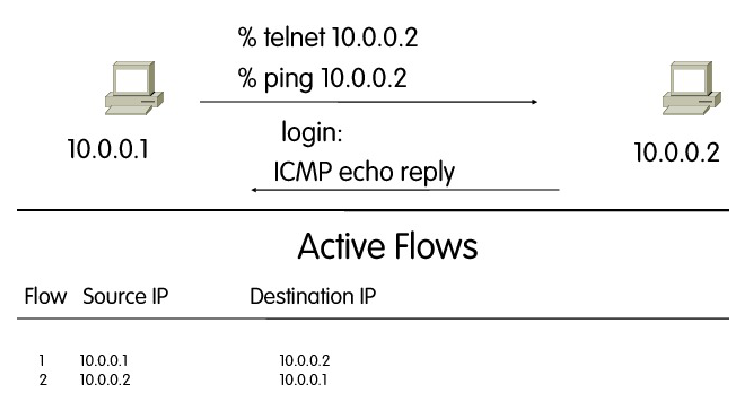
\includegraphics{figure/Flussi_unidirezionali_IP.eps}
  \caption{Flussi unidirezionali tramite indirizzo IP sorgente/destinazione}
\end{figure}

\begin{figure}[htbp]
  \centering
  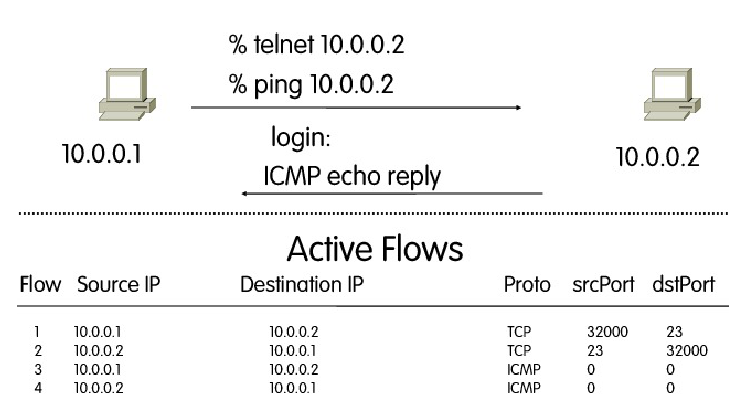
\includegraphics{figure/Flussi_unidirezionali_IP_porta_protocollo.eps}
  \caption{Flussi unidirezionali tramite indirizzo IP, porta e protocollo}
\end{figure}

\subsubsection{Aggregazione del flusso}
Vengono usati i flussi grezzi, ma spesso � necessario rispondere ad alcune domande, tipo:
\begin{itemize}
\item Quanto del traffico � web, mail, news, quake?
\item Quanto del traffico va verso o parte da un dipartimento.
\item Quanto del traffico va verso altri specifici dipartimenti, il provider X, Goolge, etc\ldots?
\item Quanto traffico passa dall'interfaccia X?
\end{itemize}

\begin{figure}[htbp]
  \centering
  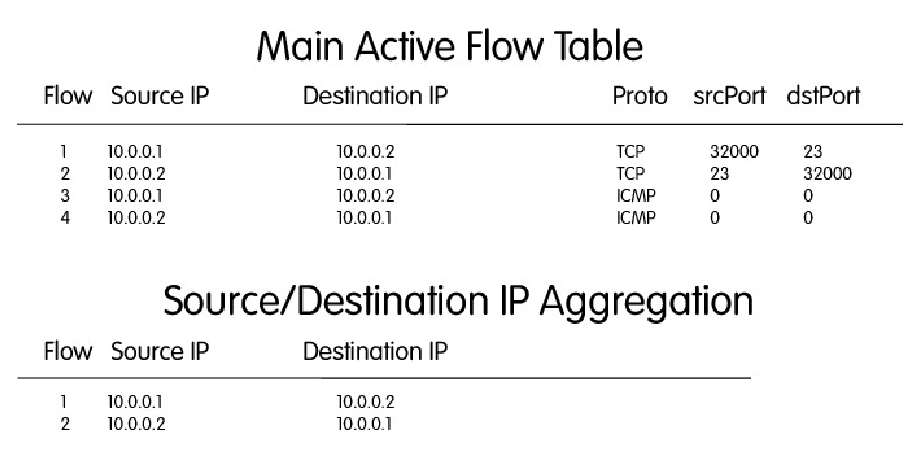
\includegraphics{figure/Aggregazione_del_flusso.eps}
  \caption{Aggregazione del flusso}
\end{figure}

Lo stesso flusso pu� essere aggregato pi� volte usando criteri differenti. Ad esempio, dai flussi grezzi � possibile generare:
\begin{itemize}
\item Lista dei protocolli.
\item Matrice delle conversazioni (chi parla con chi).
\item Le porte TCP/UDP pi� usate.
\end{itemize}

L'aggregazione del flusso � pi� veloce e usa meno memoria se viene fatta subito, piuttosto che farla dopo. Ad esempio, la matrice delle conversazioni � molto pi� semplice farla sulla sonda invece di usare grezzi flussi aggregati.

\begin{itemize}
\item I flussi possono essere aggregati usando anche criteri ``esterni'' e non solo usando i grezzi campi del flusso.
\item Generalmente questi criteri esterni sono applicati su delle ``chiavi'' (e non sui ``valori'') dei campi come una porta, l'indirizzo IP, protocollo, etc\ldots, e sono usati per raggruppare insieme i valori.
\item I criteri sono aggiunti (e non rimpiazzano) i campi esistenti.
\item Esempio: port-map, protocol-map, ip-address
  {\footnotesize
\begin{verbatim}
       IP src   IP dst   Proto Src port Dst port
Before 10.0.0.1 10.0.0.2 UDP   32000    53
       10.0.0.2 10.0.0.1 TCP   34354    80

      IP src   IP dst   Proto Src port Dst port Src port map Dst port map
After 10.0.0.1 10.0.0.2 TCP   32000    53       udp_other    domain
      10.0.0.2 10.0.0.1 TCP   34354    80       tcp_other    http
\end{verbatim}
  }
\item I flussi possono essere aggregati secondo:
  \begin{itemize}
  \item Porta TCP/UDP, \gls{ToS}, protocollo (ad esempio ICMP, UDP), \gls{AS}.
  \item IP sorgente/destinazione.
  \item Sottorete, ora del giorno.
  \end{itemize}
\item L'aggregazione pu� essere fatta sulla sonda, sul collezionatore o su entrambi.
\item L'aggregazione fatta sulla sonda � veramente efficace in termini di uso delle risorse e di flusso del traffico di rete.
\item L'aggregazione sul collezionatore � pi� potente (ad esempio aggregando i flussi prodotti da pi� sonde) ma � piuttosto costosa (riceve tutti gli aggregati).
\end{itemize}

\subsubsection{Filtrare i flussi}
Filtrare i flussi significa: scartare i flussi in base a qualche criterio come:
\begin{itemize}
\item Durata del flusso (ad esempio, scartare i flussi che non sono stati visti per pi� di X secondi).
\item Sorgente/destinazione del flusso (ad esempio, ignorare i flussi che contengono indirizzi \glstext{broadcast}).
\item Porta del flusso (ad esempio, ignorare i flussi originati sulla porta X).
\end{itemize}

Si noti che:
\begin{itemize}
\item Il filtraggio � diverso dall'aggregazione: fanno due lavori differenti.
\item Il filtraggio e l'aggregazione possono coesistere.
\item Il filtraggio viene generalmente applicato prima dell'aggregazione e non dopo.
\end{itemize}

\subsection{Architettura di NetFlow}
\begin{minipage}{.7\textwidth}
  \begin{itemize}
  \item I flussi sono esportati (push) dalla sonda quando questi finiscono, al contrario di SNMP dove il manager interroga (pull) l'agent periodicamente.
  \item Il protocollo di trasporto � NetFlow (e non SNMP).
  \item La configurazione della sonda e del collezionatore non � specificata dal protocollo NetFlow.
  \item Il collezionatore NetFlow ha il compito di assemblare e capire i flussi esportati e combinarli o aggregarli in modo da creare report significativi del traffico e per l'analisi della sicurezza.
  \end{itemize}
\end{minipage}%
\hspace{.05\textwidth}
\begin{minipage}{.23\textwidth}
  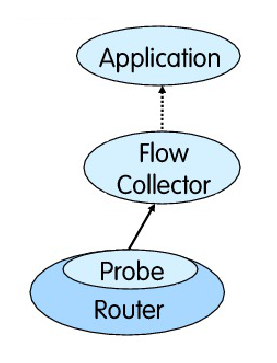
\includegraphics{figure/Architettura_NetFlow.eps}
\end{minipage}

\bigskip
Le figure \ref{architettura_NetFlow_1} e \ref{architettura_NetFlow_2} mostrano degli esempi di come si possono collezionare i dati.

\begin{figure}[htbp]
  \centering
  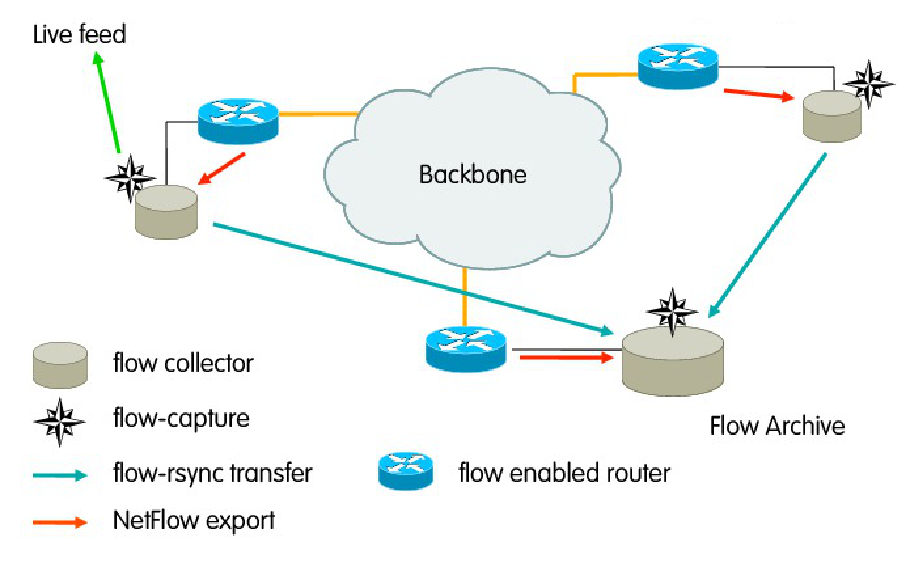
\includegraphics{figure/Flussi_architettura_collezionatore_1.eps}
  \caption{Architettura di NetFlow}
  \label{architettura_NetFlow_1}
\end{figure}

\begin{figure}[htbp]
  \centering
  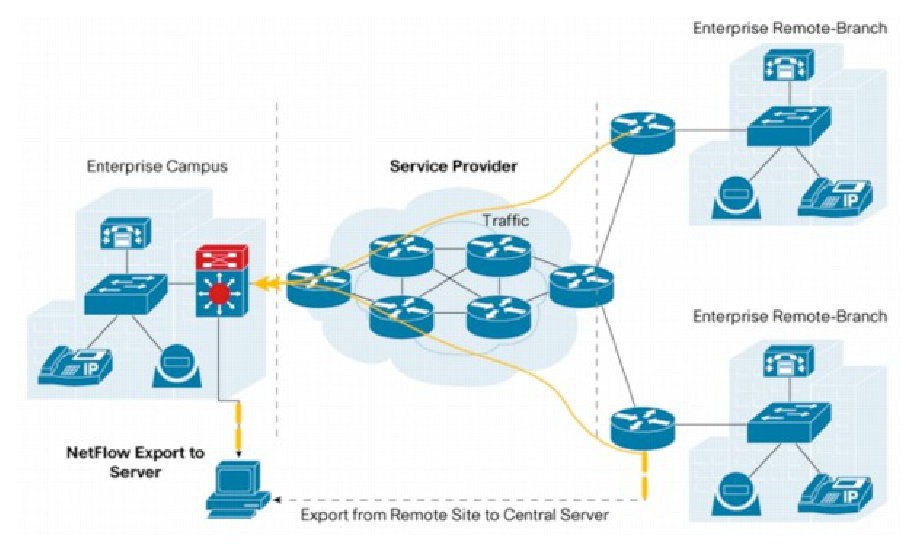
\includegraphics{figure/Flussi_architettura_collezionatore_2.eps}
  \caption{Architettura di NetFlow}
  \label{architettura_NetFlow_2}
\end{figure}

\subsubsection{Vincoli di spazio per il collezionatore}
\begin{itemize}
\item Lo spazio richiesto dipende dal traffico.
\item Qualche cifra media:
  \begin{itemize}
  \item 67.320 ottetti/flusso, 92 pacchetti/flusso.
  \item Occupazione dei router: 397 GB di traffico/giorno, 548.000.000 di pacchetti/giorno == 5.900.000 pacchetti/giorno.
  \item A 60 byte/flusso ci vogliono 350 MB di log/giorno.
  \item Con una compressione di livello 6 si ha 4.3:1.
  \item Lavoro per 82 MB/giorno per un router.
  \end{itemize}
\end{itemize}

\subsubsection{Nozioni di base per Cisco NetFlow}
\begin{itemize}
\item Flussi unidirezionali (fino alla v8), bidirezionali sulla v9.
\item Molte versioni, v1,5,6,7,8,9. La pi� comune � la v5, l'ultima � la v9.
\item Si analizza solo il traffico IP (non su tutte le piattaforme) e solo inbound (cio� il traffico che entra nel router).
\item IPv4 \glstext{unicast} e \glstext{multicast}: tutte le versioni di NetFlow. IPv6 � supportata solo dalla v9.
\item Protocollo aperto definito dalla Cisco e supportato dalle piattaforme IOS e CatIOS (nessun NetFlow � supportato dai firewall PIX) cos� come sulle piattaforme on-Cisco.
\end{itemize}

\subsubsection{Versioni di Cisco NetFlow}
\begin{itemize}
\item Ogni versione ha proprio formato per il pacchetto:
  \begin{itemize}
  \item v1,5,6,7,8 hanno un loro fissato/chiuso, specifico formato.
  \item v9 � dinamico e aperto alle estensioni.
  \end{itemize}
\item Numeri di sequenza:
  \begin{itemize}
  \item v1 non ha numeri di sequenza (nessun modo per determinare la perdita di flussi).
  \item v5,6,7,8 i numeri di sequenza per i flussi (cio� tiene traccia del numero di flussi emessi).
  \item v9 ha i numeri di sequenza per i pacchetti (no per i flusso) (cio� � facile capire il numero di pacchetti persi, ma non di flussi persi).
  \end{itemize}
\item La ``versione'' stabilisce che tipo di dato c'� nel flusso.
\item Qualche versione (ad esempio la v7) � specifico per le piattaforme Catalyst della Cisco.
\end{itemize}

\subsubsection{Netflow: nascita e morte di un flusso}
\begin{itemize}
\item Di ogni pacchetto che � stato inviato al router o ad uno switch di livello 3 viene analizzato un insieme di attributi IP.
\item Tutti i pacchetti che hanno lo stesso:
  \begin{itemize}
  \item indirizzo IP di sorgente e destinazione.
  \item porta sorgente e destinazione.
  \item protocollo.
  \end{itemize}
  sono raggruppati insieme e vengono contati sia i byte che i pacchetti.
\item I flussi attivi vengono salvati in memoria, in quella che viene chiamata, cache NetFlow.
\end{itemize}
La figura \ref{NetFlow_nascita_di_un_flusso} mostra come avviene la creazione del flusso.

\begin{figure}[htbp]
  \centering
  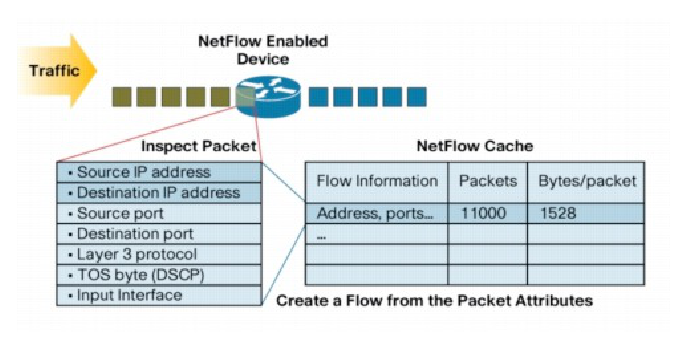
\includegraphics{figure/NetFlow_nascita_del_flusso.eps}
  \caption{NetFlow: nascita del flusso}
  \label{NetFlow_nascita_di_un_flusso}
\end{figure}

I flussi terminano quando avviene una di queste condizioni:
\begin{itemize}
\item La comunicazione � finita (ad esempio la comunicazione contiene il flag TCP FIN o RST).
\item \`E durato troppo (di default 30 minuti).
\item Il flusso non � pi� attivo (non sono stati ricevuti pacchetti) da troppo tempo (di default 15 secondi).
\item La cache NetFlow � piena e il gestore della cache deve eliminare qualche dato.
\end{itemize}
Si noti che la cache NetFlow ha una dimensione limitata, quindi spesso non � possibile inserirvi tutti i flussi (si veda la figura \ref{NetFlow_cache_dei_flussi}).

\begin{figure}[htbp]
  \centering
  
\includegraphics{figure/NetFlow_cache_dei_flussi.eps}
  \caption{NetFlow: politiche di esportazione dei flussi dalla cache NetFlow}
  \label{NetFlow_cache_dei_flussi}
\end{figure}

\begin{itemize}
\item La cache NetFlow si riempie costantemente di flussi, quindi il software all'interno del router o dello switch va in cerca di quei flussi che sono terminati o scaduti e li esporta verso il collezionatore.
\item Una conseguenza � che il flusso di rete viene spezzato in molti flussi NetFlow che, se necessario, vengono riassemblati dal collezionatore.
\end{itemize}

\subsubsection{Formato del pacchetto del flusso}
\begin{itemize}
\item Un header comune tra le versioni esportate.
\item Vengono esportati N record e la versione specifica cosa contengono.
\item N viene determinato dalla definizione del flusso (ad esempi N=30 per v5). La dimensione del pacchetto viene mantenuta sotto i 1480 byte circa in modo da non avere nessuna frammentazione a livello ethernet.
\end{itemize}
\begin{figure}[htbp]
  \centering
  
\includegraphics{figure/NetFlow_pacchetto_v5.eps}
  \caption{Pacchetto NetFlow v5}
\end{figure}

\subsection{Cisco NetFlow v5}

{\footnotesize
\begin{verbatim}
    struct netflow5_record {
      struct flow_ver5_hdr flowHeader;
      struct flow_ver5_rec flowRecord[30];
    } NetFlow5Record;

    struct flow_ver5_hdr {
      u_int16_t version;                 /* Current version=5*/
      u_int16_t count;                   /* The number of records in PDU. */
      u_int32_t sysUptime;               /* Current time in msecs since router booted */
      u_int32_t unix_secs;               /* Current seconds since 0000 UTC 1970 */
      u_int32_t unix_nsecs;              /* Residual nanoseconds since 0000 UTC 1970 *
      u_int32_t flow_sequence;           /* Sequence number of total flows seen */
      u_int8_t engine_type;              /* Type of flow switching engine (RP,VIP,etc.)*/
      u_int8_t engine_id;                /* Slot number of the flow switching engine */

      struct flow_ver5_rec {
        u_int32_t srcaddr;   /* Source IP Address */
        u_int32_t dstaddr;   /* Destination IP Address */
        u_int32_t nexthop;   /* Next hop router's IP Address */
        u_int16_t input;     /* Input interface index */
        u_int16_t output;    /* Output interface index */
        u_int32_t dPkts;     /* Packets sent */
        u_int32_t dOctets;   /* Octets sent */
        u_int32_t First;     /* SysUptime at start of flow */
        u_int32_t Last;      /* and of last packet of the flow */
        u_int16_t srcport;   /* TCP/UDP source port number (.e.g, FTP, Telnet, etc.,or equivalent) */
        u_int16_t dstport;   /* TCP/UDP destination port number (.e.g, FTP, Telnet, etc.,or equivalent) */
        u_int8_t pad1;       /* pad to word boundary */
        u_int8_t tcp_flags;  /* Cumulative OR of tcp flags */
        u_int8_t prot;       /* IP protocol, e.g., 6=TCP, 17=UDP, etc... */
        u_int8_t tos;        /* IP Type-of-Service */
        u_int16_t src_as;    /* source peer/origin Autonomous System */
        u_int16_t dst_as;    /* dst peer/origin Autonomous System */
        u_int8_t src_mask;   /* source route's mask bits */
        u_int8_t dst_mask;   /* destination route's mask bits */
        u_int16_t pad2;      /* pad to word boundary */
      };
\end{verbatim}
}

\subsection{NetFlow v9}
\subsubsection{Perch� se ne ha bisogno?}
\begin{itemize}
\item I formati fissi (dalla versione 1 alla 8) sono:
  \begin{itemize}
  \item Facili da implementare.
  \item Consumano poca larghezza di banda.
  \item Sono facili da decifrare per il collezionatore.
  \item Non flessibili (molti ???)
  \item Non estensibili (non c'� modo di estendere il flusso a meno che non venga definita una nuova versione).
  \item Qualche caratteristica viene persa: livello 2, VLAN, IPv6, MPLS\footnote{Multiprotocol Label Switching (MPLS) � un meccanismo delle reti performanti che dirige e trasporta i dati direttamente da un nodo della rete ad un altro. MPLS rende facile la creazione di ``link virtuali'' tra due nodi distanti. \`E in grado di incapsulare vari tipi di protocolli.}.
  \end{itemize}
\end{itemize}

\subsubsection{I principi}
\begin{itemize}
\item Protocollo aperto definito da Cisco (non � proprietario) nelle RFC 3954.
\item Template di flusso + record di flusso
  \begin{itemize}
  \item Il template � composto da tipo e lunghezza.
  \item Il record di un flusso � composto da un template ID e da un valore.
  \item I template sono spediti periodicamente e sono il prerequisito per decodificare i record del flusso.
  \item I record del flusso contengono ``la ciccia''.
  \end{itemize}
\item Template di opzioni + record di opzioni, contengono la configurazione della sonda (ad esempio, la velocit� di campionamento, interfaccia dei pacchetti).
\item Modello push della sonda verso il collezionatore (come nelle precedenti versioni).
\item Spedisce i template regolarmente: ogni X flussi, ogni X secondi.
\item Indipendente dal protocollo sottostante, pronto per ogni protocollo affidabile.
\item Pu� spedire sia i template che i record di flusso in una sola esportazione.
\item Pu� inserire differenti record di flussi in una sola esportazione.
\end{itemize}

\begin{figure}[htbp]
  \centering
  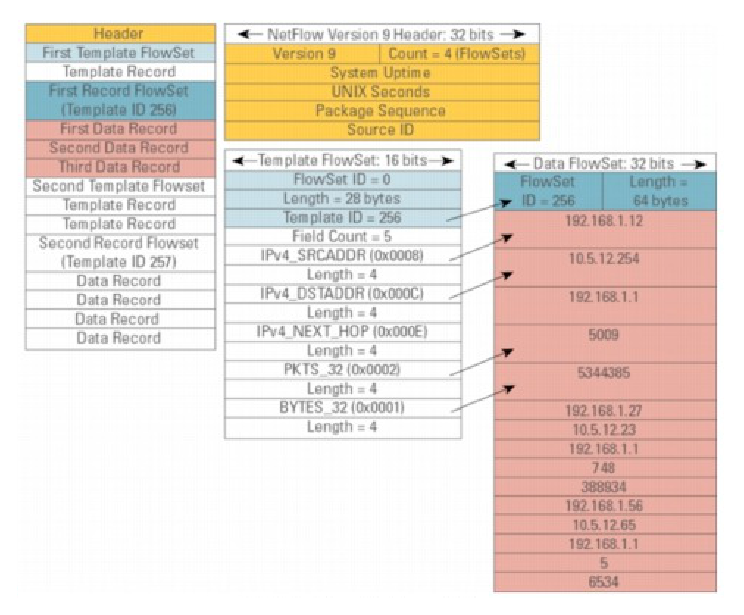
\includegraphics{figure/NetFlow_v9_formato.eps}
  \caption{Formato di NetFlow v9}
\end{figure}

\subsubsection{Qualche tag}

{\footnotesize
\begin{verbatim}
[ 1] %IN_BYTES                Incoming flow bytes
[ 2] %IN_PKTS                 Incoming flow packets
[ 3] %FLOWS                   Number of flows
[ 4] %PROTOCOL                IP protocol byte
[ 5] %SRC_TOS                 Type of service byte
[ 6] %TCP_FLAGS               Cumulative of all flow TCP flags
[ 7] %L4_SRC_PORT             IPv4 source port
[ 8] %IPV4_SRC_ADDR           IPv4 source address
[ 9] %SRC_MASK                Source subnet mask (/<bits>)
[ 10] %INPUT_SNMP             Input interface SNMP idx
[ 11] %L4_DST_PORT            IPv4 destination port
[ 12] %IPV4_DST_ADDR          IPv4 destination address
[ 13] %DST_MASK               Dest subnet mask (/<bits>)
[ 16] %SRC_AS                 Source BGP AS
[ 17] %DST_AS                 Destination BGP AS
[ 21] %LAST_SWITCHED          SysUptime (msec) of the last flow pkt
[ 22] %FIRST_SWITCHED         SysUptime (msec) of the first flow pkt
[ 23] %OUT_BYTES              Outgoing flow bytes
[ 24] %OUT_PKTS               Outgoing flow packets
[ 27] %IPV6_SRC_ADDR          IPv6 source address
[ 28] %IPV6_DST_ADDR          IPv6 destination address
[ 29] %IPV6_SRC_MASK          IPv6 source mask
[ 30] %IPV6_DST_MASK          IPv6 destination mask
[ 32] %ICMP_TYPE              ICMP Type * 256 + ICMP code
[ 34] %SAMPLING_INTERVAL      Sampling rate
[ 37] %FLOW_INACTIVE_TIMEOUT  Inactivity timeout of flow cache entries
[ 38] %ENGINE_TYPE            Flow switching engine
[ 39] %ENGINE_ID              Id of the flow switching engine
[ 40] %TOTAL_BYTES_EXP        Total bytes exported
[ 41] %TOTAL_PKTS_EXP         Total flow packets exported
[ 42] %TOTAL_FLOWS_EXP        Total number of exported flows
[ 56] %IN_SRC_MAC             Source MAC Address
[ 57] %OUT_DST_MAC            Destination MAC Address
[ 58] %SRC_VLAN               Source VLAN
[ 59] %DST_VLAN               Destination VLAN
[ 60] %IP_PROTOCOL_VERSION    [4=IPv4][6=IPv6]
[ 70] %MPLS_LABEL_1           MPLS label at position 1
[ 71] %MPLS_LABEL_2           MPLS label at position 2
[ 72] %MPLS_LABEL_3           MPLS label at position 3
[ 73] %MPLS_LABEL_4           MPLS label at position 4
[ 74] %MPLS_LABEL_5           MPLS label at position 5
[ 75] %MPLS_LABEL_6           MPLS label at position 6
[ 76] %MPLS_LABEL_7           MPLS label at position 7
[ 77] %MPLS_LABEL_8           MPLS label at position 8
[ 78] %MPLS_LABEL_9           MPLS label at position 9
[ 79] %MPLS_LABEL_10          MPLS label at position 10
[ 80] %IN_DST_MAC             Source MAC Address
[ 81] %OUT_SRC_MAC            Destination MAC Address
\end{verbatim}
}

\subsubsection{Esempio}

{\footnotesize
\begin{verbatim}
Cisco NetFlow
    Version: 9
    Count: 4
    SysUptime: 1132427188
    Timestamp: Aug 18, 2000 23:49:25.000012271
        CurrentSecs: 966635365
    FlowSequence: 12271
    SourceId: 0
    FlowSet 1/4
 FlowSet 1/4
        Template FlowSet: 0
        FlowSet Length: 164
        Template Id: 257
        Field Count: 18
        Field (1/18)
            Type: LAST_SWITCHED (21)
            Length: 4

Cisco NetFlow
    Version: 9
    Count: 1
    SysUptime: 1133350352
    Timestamp: Aug 19, 2000 00:04:48.000012307
        CurrentSecs: 966636288
    FlowSequence: 12307
    SourceId: 0
    FlowSet 1/1
        Data FlowSet (Template Id): 257
        FlowSet Length: 52
        pdu 1
            EndTime: 1133334.000000000 seconds
            StartTime: 1133334.000000000 seconds
            Octets: 84
            Packets: 1
            InputInt: 15
\end{verbatim}
}

\subsubsection{Template di opzioni}
\begin{figure}[htbp]
  \centering
  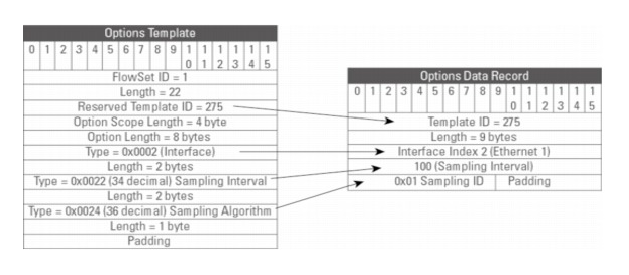
\includegraphics{figure/NetFlow_v9_template_di_opzioni.eps}
  \caption{NetFlow v9: template di opzioni}
\end{figure}

\subsubsection{v5 contro v9}
\begin{tabular}{|l|l|l|}
  \hline
  & v5 & v9\\
  \hline
  Formato del flusso & Fisso & Definito dall'utente\\
  \hline
  Estensibile & No & Si (definendo un nuovo campo FlowSet)\\
  \hline
  Tipo di flusso & Unidirezionale & Bidirezionale\\
  \hline
  Dimensione del flusso & 48 byte (fisso) & Dipende dal formato\\
  \hline
  IPv6 & No & IPv4 e IPv6\\
  \hline
  MPLS/VLAN & No & Si\\
  \hline
\end{tabular}

\subsection{Cisco IOS}
\subsubsection{Configurazione}
\begin{itemize}
\item Configurato su ogni interfaccia di input.
\item Definire la versione.
\item Definire l'indirizzo IP del collezionatore (dove esportare i flussi).
\item Opzionalmente abilita l'aggregazione delle tabelle.
\item Opzionalmente configura il timeout del flusso e la principale (v5) dimensione della tabella di flusso.
\item Opzionalmente configura la velocit� di campionamento.
\end{itemize}

{\footnotesize
\begin{verbatim}
interface FastEthernet0/0/0
 ip address 10.0.0.1 255.255.255.0
 no ip directed-broadcast
 ip route-cache flow

interface ATM1/0/0
 no ip address
 no ip directed-broadcast
 ip route-cache flow

interface Loopback0
 ip address 10.10.10.10 255.255.255.255
 no ip directed-broadcast

ip flow-export version 5 origin-as
ip flow-export destination 10.0.0.10 5004
ip flow-export source loopback 0

ip flow-aggregation cache prefix
 export destination 10.0.0.10 5555
 enabled
\end{verbatim}
}

\subsubsection{Report}

{\footnotesize
\begin{verbatim}
#sh ip flow export
Flow export is enabled
  Exporting flows to 10.0.0.10 (5004)
  Exporting using source IP address 10.10.10.10
  Version 5 flow records, origin-as
  Cache for prefix aggregation:
    Exporting flows to 10.0.0.10 (5555)
    Exporting using source IP address 10.10.10.10
  3176848179 flows exported in 105898459 udp datagrams
  0 flows failed due to lack of export packet
  45 export packets were sent up to process level
  0 export packets were punted to the RP
  5 export packets were dropped due to no fib
  31 export packets were dropped due to adjacency issues
  0 export packets were dropped due to fragmentation failures
  0 export packets were dropped due to encapsulation fixup failures
  0 export packets were dropped enqueuing for the RP
  0 export packets were dropped due to IPC rate limiting
  0 export packets were dropped due to output drops

#sho ip ca fl
IP packet size distribution (106519M total packets):
   1-32    64   96  128  160  192  224  256  288  320  352  384  416  448  480
   .002  .405 .076 .017 .011 .010 .007 .005 .004 .005 .004 .004 .003 .002 .002

    512  544  576 1024 1536 2048 2560 3072 3584 4096 4608
   .002 .006 .024 .032 .368 .000 .000 .000 .000 .000 .000

IP Flow Switching Cache, 4456704 bytes
  36418 active, 29118 inactive, 3141073565 added
  3132256745 ager polls, 0 flow alloc failures
  Active flows timeout in 30 minutes
  Inactive flows timeout in 15 seconds
  last clearing of statistics never
Protocol          Total   Flows   Packets Bytes Packets Active(Sec) Idle(Sec)
--------          Flows    /Sec     /Flow  /Pkt      /Sec    /Flow     /Flow
TCP-Telnet      2951815     0.6        61   216      42.2     26.6      21.4
TCP-FTP        24128311     5.6        71   748     402.3     15.0      26.3
TCP-FTPD        2865416     0.6       916   843     611.6     34.7      19.8
TCP-WWW       467748914   108.9        15   566    1675.8      4.9      21.6
TCP-SMTP       46697428    10.8        14   370     159.6      4.0      20.1
TCP-X            521071     0.1       203   608      24.7     24.5      24.2
TCP-BGP         2835505     0.6         5    94       3.3     16.2      20.7
TCP-other    1620253066   377.2        47   631   18001.6     27.3      23.4
UDP-DNS       125622144    29.2         2    78      82.5      4.6      24.7
UDP-NTP        67332976    15.6         1    76      22.0      2.7      23.4
UDP-TFTP          37173     0.0         2    76       0.0      4.1      24.6
UDP-Frag          68421     0.0       474   900       7.5    111.7      21.6
UDP-other     493337764   114.8        17   479    1990.3      3.8      20.2
ICMP          243659509    56.7         3   166     179.7      3.3      23.3
IGMP              18601     0.0        96    35       0.4    941.4       8.1
IPINIP            12246     0.0        69    52       0.1    548.4      15.2
GRE              125763     0.0       235   156       6.9     50.3      21.1
IP-other       75976755    17.6         2    78      45.4      3.9      22.8
Total:       3176854246   739.6        33   619   24797.4     16.2      22.6

SrcIf         SrcIPaddress     DstIf        DstIPaddress   Pr  SrcP DstP   Pkts
AT5/0/0.4     206.21.162.150   AT1/0/0.1    141.219.73.45  06  0E4B A029    507
AT4/0/0.10    132.235.174.9    AT1/0/0.1    137.99.166.126 06  04BE 074C      3
AT4/0/0.12    131.123.59.33    AT1/0/0.1    137.229.58.168 06  04BE 09BB    646
AT1/0/0.1     137.99.166.126   AT4/0/0.10   132.235.174.9  06  074C 04BE      3

#show ip flow top-talkers
SrcIf SrcIPaddress DstIf DstIPaddress Pr SrcP DstP Pkts
Et1/0  172.16.10.2 Et0/0  172.16.1.84 06 0087 0087 2100
Et1/0  172.16.10.2 Et0/0  172.16.1.85 06 0089 0089 1892
Et1/0  172.16.10.2 Et0/0  172.16.1.86 06 0185 0185 1762
Et1/0  172.16.10.2 Et0/0  172.16.1.86 06 00B3 00B3 2
Et1/0  172.16.10.2 Et0/0  172.16.1.84 06 0050 0050 1
Et1/0  172.16.10.2 Et0/0  172.16.1.85 06 0050 0050

17 of 10 top talkers shown. 7 flows processed.

#show ip flow top 10 aggregate destination-address
There are 3 top talkers:
IPV4 DST-ADDR        bytes       pkts      flows
=============== ========== ========== ==========
172.16.1.86            160          4          2
172.16.1.85            160          4          2
172.16.1.84            160          4          2

#show ip flow top 10 aggregate destination-address sorted-by bytes match
source-port min 0 max 1000
There are 3 top talkers:
IPV4 DST-ADDR        bytes       pkts      flows
=============== ========== ========== ==========
172.16.1.84             80          2          2
172.16.1.85             80          2          2
172.16.1.86             80          2         26 of 6 flows matched.
\end{verbatim}
}

\subsection{Configurazione JunOS}
\begin{itemize}
\item Pacchetti campione filtrati da un firewall e inviati verso un motore di routing.
\item La velocit� di campionamento � limitata a 7000pps (packets per seconds) indirizzati al prossimo PIC (Physical Interface Card).
\item Buono per il controllo del traffico, ma non troppo efficace per scoprire attacchi \gls{DoS} o le intrusioni.
\item Juniper \footnote{JunOS � un sistema operativo di rete affidabile e ad alte prestazioni per router, switch e dispositivi di sicurezza sviluppato da Juniper.} chiama NetFlow cflowd (un popolare collezionatore fornito dalla CAIDA).
\end{itemize}

\begin{tabular}{p{0.2\textwidth}|p{0.35\textwidth}|p{0.35\textwidth}}
  {\bf Filtri per il firewall}
  {\footnotesize
\begin{verbatim}
firewall {
  filter all {
    term all {
      then {
        sample;
        accept;
      }
    }
  }
}
\end{verbatim}
  }
  &
  {\bf Abilitare il campionamento/flusso}
  {\footnotesize
\begin{verbatim}
forwarding-options {
  sampling {
    input {
      family inet {
        rate 100;
      }
    }
    output {
      cflowd 10.0.0.16{
        port 2055;
        version 5;
      }
    }
  }
}
\end{verbatim}
  }
  &
  {\bf Applicare i filtri del firewall ad ogni interfaccia}
  {\footnotesize
\begin{verbatim}
interfaces {
  ge-0/3/0 {
    unit 0 {
      family inet {
        filter {
          input all;
          output all;
        }
        address 192.148.244.1/24;
      }
    }
  }
\end{verbatim}
  }
\end{tabular}

\subsection{Sonde NetFlow basate sui PC}
\begin{itemize}
\item Ci sono  sonde NetFlow basate sui PC.
\item Molte di queste si basano sulla libreria pcap.
\item nProbe (\url{www.ntop.org/nProbe.html}):
  \begin{itemize}
  \item Open Source (GPL2).
  \item Una sonda veloce sul mercato.
  \item Supporta sia NetFlow v5,v9 che IPFIX.
  \item Formato flessibile per i flussi esportati.
  \item Supporta IPv4/v6, un template flessibile (non sempre supportato da Cisco).
  \item Disponibile sia per Linux che per Windows.
  \end{itemize}
\end{itemize}

\subsection{IPFIX}
\subsubsection{Campo di applicazione e requisiti generali}
\begin{itemize}
\item Scopo: trovare o sviluppare una base comune per la misurazione del flusso di traffico IP in modo che sia disponibile su (quasi) tutti i router futuri.
\item Requisiti che soddisfano molte applicazioni.
\item Basso costo hardware/software.
\item Semplice e scalabile.
\item Dovrebbe essere integrabile su tutti i router IP e altri dispositivi (sonde o middle boxe\footnote{I middle boxe sono quei dispositivi che si trovano nel mezzo del traffico, come appunto i router, switch, etc\ldots.}).
\item Processare i dati in modo che sia integrato su varie applicazioni.
\item Interoperabilit� sia nell'apertura che nella standardizzazione.
\end{itemize}

\subsubsection{In breve}
\begin{itemize}
\item Fortemente basato su NetFlow v9.
\item Capacit� di definire nuovi campi per il flusso usando un formato standard (OID).
\item Il trasporto del flusso � basato su SCTP (Stream Control Transport Protocol), opzionalmente su supporto UDP/TCP.
\item Stato corrente: bozza della specifica di protocollo.
\item In pratica: IPFIX = NetFlow v9 su SCTP.
\end{itemize}

\begin{figure}[htbp]
  \centering
  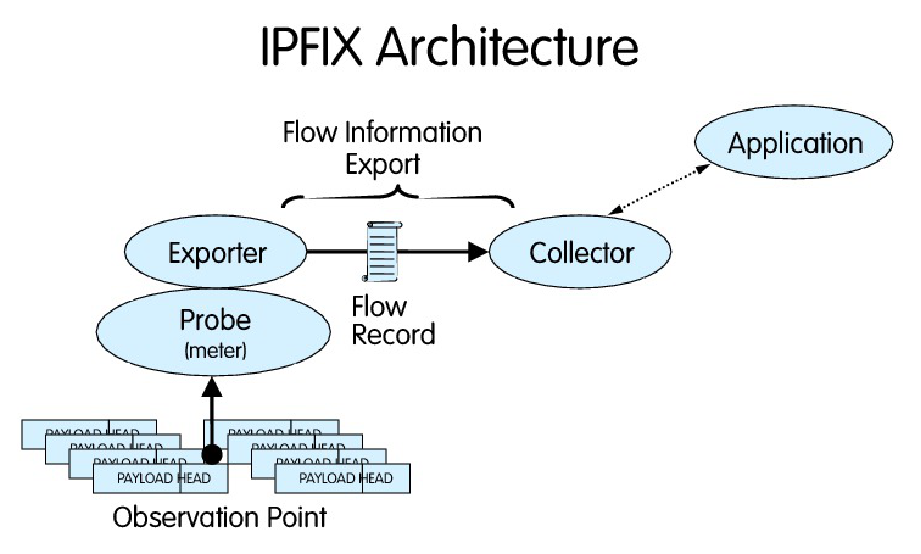
\includegraphics{figure/Architettura_IPFIX.eps}
  \caption{Architettura di IPFIX}
\end{figure}

\subsection{Flussi e sicurezza}
NetFlow e IPFIX possono essere usati anche a livello di sicurezza e non solo per la gestione del traffico:
\begin{itemize}
\item Possono individuare portscan\footnote{Si scansionano tutte le porte alla ricerca dei servizi attivi.}/portmap\footnote{Scovare un host con il servizio RPC (Remote Procedure Call) attivo. Questo servizio permette di eseguire delle elaborazioni remote.}.
\item Scovare attivit� su porte sospette.
\item Identificare la sorgente di uno SPAM, disabilitare i server (ad esempio un server file).
\end{itemize}

\subsubsection{Portmap}

{\footnotesize
\begin{verbatim}
Start       SrcIPaddress    SrcP DstIPaddress DstP P Pkts
10:53:42.50 165.132.86.201  9781 128.146.0.76  111 6    1
10:53:42.54 165.132.86.201  9874 128.146.0.7   111 6    1
10:53:42.54 165.132.86.201  9982 128.146.0.80  111 6    1
10:53:42.54 165.132.86.201  9652 128.146.0.74  111 6    1
10:53:42.54 165.132.86.201  9726 128.146.0.75  111 6    1
10:53:42.54 165.132.86.201  9855 128.146.0.77  111 6    1
10:53:42.58 165.132.86.201 10107 128.146.0.82  111 6    1
\end{verbatim}
}
In un breve lasso di tempo ci sono molti pacchetti con lo stesso indirizzo sorgente ma con differenti indirizzi di destinazione e tutti sulla stessa porta di destinazione (porta 111=RPC (Remote Procedure Call)).

\subsubsection{Trovare le backdoor}

{\footnotesize
\begin{verbatim}
Start    SrcIPaddress   SrcP DstIPaddress    DstP P Pkts
19:08:40 165.132.86.201 8401 128.146.172.232 1524 6  19
19:08:40 165.132.86.201 8422 128.146.172.230 1524 6  16
19:08:40 165.132.86.201 8486 128.146.172.234 1524 6  19
19:08:40 165.132.86.201 8529 128.146.172.236 1524 6  10
19:08:41 165.132.86.201 8614 128.146.172.237 1524 6  16
19:08:41 165.132.86.201 8657 128.146.172.238 1524 6  22
\end{verbatim}
}

Come il portmap, solo si cercano porte aperte da applicazioni conosciute, nell'esempio la porta di destinazione � la 1524 (trinoo backdoor port \url{http://www.auditmypc.com/port/tcp-port-1524.asp}).

\subsubsection{Trovare le intrusioni}
Semplice sistema IDS\footnote{Intrusion Detection System} basato sui flussi:
\begin{itemize}
\item I flussi che hanno troppi ottetti o troppi pacchetti (troppi dati: floods - inondazione).
\item Lo stesso IP sorgente contatta pi� di N destinazioni - host scanning.
\item Lo stesso IP sorgente contatta pi� di M porte per la stessa destinazione - port scanning.
\end{itemize}

% LocalWords:  SNMP agent L'agent trap polling Get dall'agent collezionatori of
% LocalWords:  MIB Cisco NetFlow UDP collezionatore L'instrumentazione offline
% LocalWords:  router switch ASN Autonomous System Number routing BGP Border AS
% LocalWords:  Gateway Protocol SMTP sharing DoS Denial Service com host TCP ip
% LocalWords:  NetBIOS AppleTalk firewall RST IPFIX Flow Information IETF trip
% LocalWords:  Overhead VLAN news quake Goolge esterni' chiavi' valori' port GB
% LocalWords:  map protocol address ToS Type ICMP Sottorete broadcast push pull
% LocalWords:  l'agent report Reader' NeTraMet RFC MB log inbound IPv unicast
% LocalWords:  multicast
% LocalWords:  IOS CatIOS PIX Catalyst Netflow cache header ethernet MPLS Label
% LocalWords:  Multiprotocol Switching virtuali' Template template tag FlowSet
% LocalWords:  JunOS pps packets seconds PIC Physical Interface Juniper cflowd
% LocalWords:  CAIDA pcap nProbe Source middle OID SCTP Stream Control portscan
% LocalWords:  Transport portmap RPC Call SPAM backdoor trinoo IDS Intrusion
% LocalWords:  Detection floods scanning

\section{sFlow}
\subsection{sFlow}
\subsubsection{Principi}
\begin{itemize}
\item Non si pretenda di essere veloce come la rete che si vuole monitorare: si perderanno comunque dei dati.
\item Anche se si riesce a monitorare tutto, si avranno comunque delle difficolt� nel gestire tutti i flussi generati.
\item Analizzare 1 pacchetto ogni X pacchetti (campionamento).
\item Pi� pacchetti si analizza, pi� si avranno dati precisi.
\item Se la rete � troppo veloce, si aumenta il valore di campionamento.
\end{itemize}

\subsubsection{Architettura}
\begin{minipage}{.58\textwidth}
  \begin{itemize}
  \item La sonda campiona il traffico.
  \item I pacchetti campione sono spediti (nel formato sFlow) al collezionatore.
  \item Periodicamente la sonda invia le statistiche raccolte sulle interfacce (i contatori MIB II SNMP) dentro i pacchetti sFlow.\\
    I pacchetti sono usati per ``scalare'' il traffico.
  \end{itemize}
\end{minipage}
\hspace{.05\textwidth}
\begin{minipage}{.27\textwidth}
  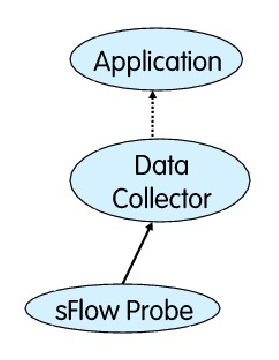
\includegraphics{figure/Architettura_sFlow.eps}
\end{minipage}

\subsubsection{Specifiche}
\begin{itemize}
\item Specificato nelle RFC 3176 (RFC informative) proposte dalla InMon Inc..
\item Definisce:
  \begin{itemize}
  \item Formato del pacchetto sFlow (UDP, no SNMP).
  \item Un MIB SNMP per accedere ai dati sFlow raccolti\\
    (\url{http://support.ipmonitor.com/mibs/SFLOW-MIB/tree.aspx}).
  \end{itemize}
\item L'architettura di sFlow � simile a quella di NetFlow: la sonda spedisce i pacchetti sFlow al collezionatore.
\item La sonda sFlow � in pratica uno sniffer che cattura 1 pacchetto su X (la proporzione di default � 1:400).
\item Questi pacchetti sono spediti al collezionatore codificati nel formato sFlow.
\item Periodicamente la sonda spedisce altri pacchetti sFlow che contengono statistiche sulle interfacce di rete (ad esempio i contatori del traffico dell'interfaccia), statistiche che sono usate per scalare i dati raccolti.
\item Usando delle formule statistiche � possibile produrre un rapporto abbastanza preciso del traffico.
\item $\%Errore\ di\ campionamento \le 196 \times \sqrt{\frac{1}{numero\ di\ campioni}}$
  \bigskip \\
  \url{http://www.sflow.org/packetSamplingBasics/}.
\item sFlow � scalabile (basta incrementare il rapporto di campionamento) anche sulle 10 GB e oltre.
\item ntop.org � parte del consorzio sFlow.org.
\end{itemize}

\subsubsection{Il pacchetto}

{\footnotesize
\begin{verbatim}
struct sample_datagram_v5 {
   address agent_address          /* IP address of sampling agent,
                                     sFlowAgentAddress. */
   unsigned int sub_agent_id;     /* Used to distinguishing between datagram
                                     streams from separate agent sub entities
                                     within an device. */
   unsigned int sequence_number;  /* Incremented with each sample datagram
                                     generated by a sub-agent within an
                                     agent. */
   unsigned int uptime;           /* Current time (in milliseconds since device
                                     last booted). Should be set as close to
                                     datagram transmission time as possible.
                                     Note: While a sub-agents should try and
                                           track the global sysUptime value
                                           a receiver of sFlow packets must
                                           not assume that values are
                                           synchronised between sub-agents. */
   sample_record samples<>;        /* An array of sample records */
}

struct flow_sample {
   unsigned int sequence_number;  /* Incremented with each flow sample
                                     generated by this source_id.
                                     Note: If the agent resets the
                                           sample_pool then it must
                                           also reset the sequence_number.*/
   sflow_data_source source_id;   /* sFlowDataSource */
   unsigned int sampling_rate;    /* sFlowPacketSamplingRate */
   unsigned int sample_pool;      /* Total number of packets that could have
                                     been sampled (i.e. packets skipped by
                                     sampling process + total number of
                                     samples) */
   unsigned int drops;            /* Number of times that the sFlow agent
                                     detected that a packet marked to be
                                     sampled was dropped due to
                                     lack of resources. The drops counter
                                     reports the total number of drops
                                     detected since the agent was last reset.
                                     A high drop rate indicates that the
                                     management agent is unable to process
                                     samples as fast as they are being
                                     generated by hardware. Increasing
                                     sampling_rate will reduce the drop
                                     rate. Note: An agent that cannot
                                     detect drops will always report
                                     zero. */

   interface input;               /* Interface packet was received on. */
   interface output;              /* Interface packet was sent on. */

   flow_record flow_records<>;    /* Information about a sampled packet */
}
\end{verbatim}
}

\begin{figure}[htbp]
  \centering
  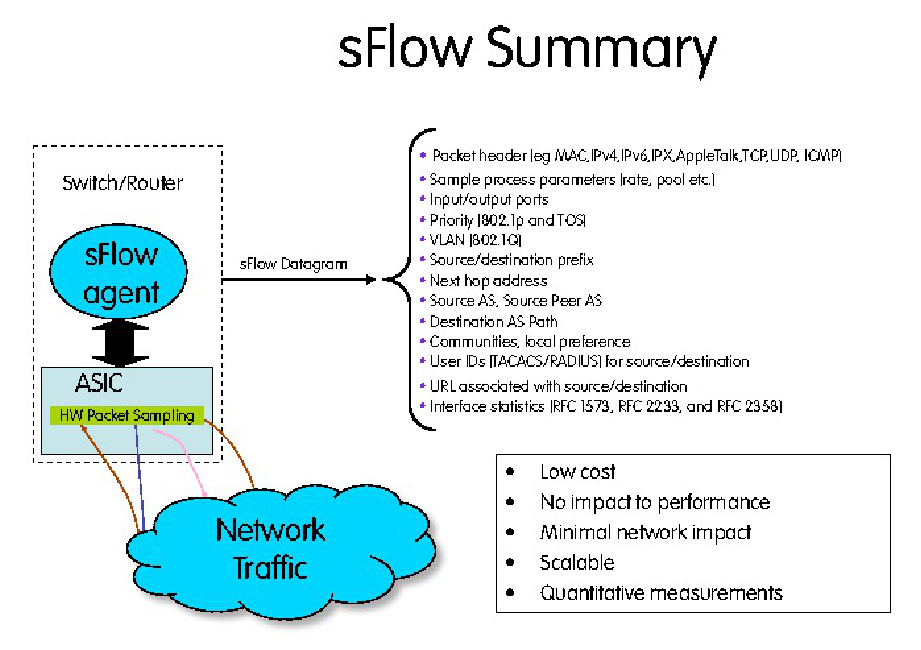
\includegraphics{figure/sFlow_sommario.eps}
  \caption{sFlow: sommario}
\end{figure}

\begin{figure}[htbp]
  \centering
  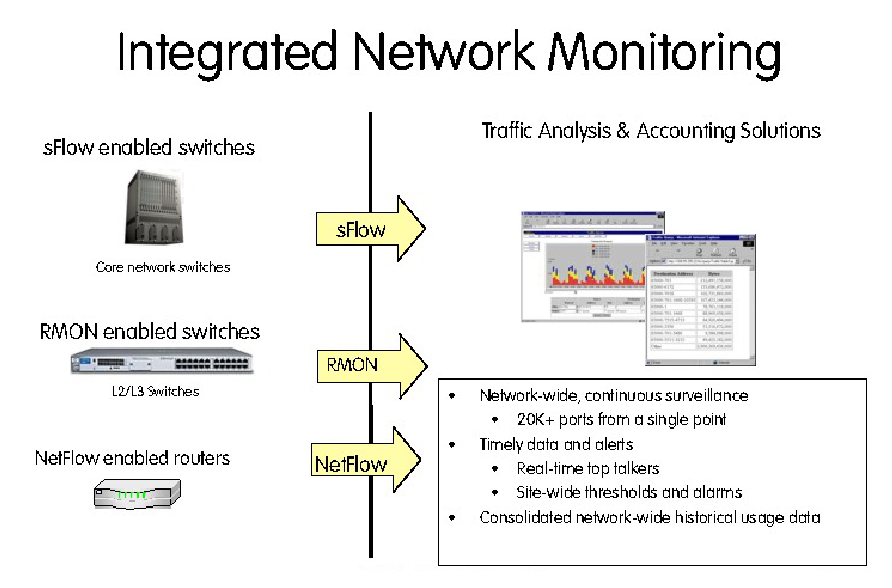
\includegraphics{figure/sFlow_monitoraggio_di_rete_integrato.eps}
  \caption{Monitoraggio di rete integrato}
\end{figure}

\subsubsection{sFlow verso NetFlow}
\begin{tabular}{|l|c|c|}
  \hline
  & sFlow & NetFlow\\
  \hline
  Ambiente nativo & Switch & Router\\
  \hline
  Velocit� a cui pu� operare & Multigigabit & 1 GB o meno\\
  \hline
  Campionamento & Sempre & Qualche volta\\
  \hline
  Monitoraggio & Statistico & Accurato (nessuna perdita)\\
  \hline
\end{tabular}

\subsection{RADIUS [RFC 2139, 1997]}
RADIUS � l'acronimo di  Remote Authentication Dial In User Service, specificato nelle seguenti RFC:
\begin{itemize}
\item Protocollo di autenticazione\\
  Rigney, C., Rubens, A., Simpson, W, and Willens, S.; Remote Authentication Dial In User Service (RADIUS), RFC 2138, January 1997.
\item Gestione dei dati\\
  Rigney, C.; RADIUS Accounting, RFC 2139, January 1997.
\end{itemize}

\subsubsection{RADIUS}
RADIUS � importante perch�:
\begin{itemize}
\item \`E il protocollo pi� usato per implementare l'autenticazione sui dispositivi di rete.
\item Usato per la fatturazione sulle reti cablate (wired lines) (ad esempio ADSL, Modem).
\item Abilita la gestione della durata della connessione o della quantit� di dati.
\item Supportato da tutti i dispositivi di rete (esclusi quelli di basso costo).
\end{itemize}

\subsubsection{Protocollo: le primitive}
La figura \ref{RADIUS} mostra un esempio di come il client RADIUS (il server per i clienti che intendono utilizzare la rete) e il server RADIUS (il server che gestisce gli account dei clienti) si scambiano i messaggi al fine di autenticare un cliente. Se il server RADIUS risponde positivamente alla richiesta di accounting, allora il cliente � libero di utilizzare la rete, altrimenti il client RADIUS gli nega l'accesso.
\bigskip

Access Request ($client \rightarrow server$):
\begin{itemize}
\item Richiesta per accedere al servizio di rete (ad esempio autenticazione dell'utente).
\item Possibile risposta:
  \begin{itemize}
  \item Access Accept ($server \rightarrow client$).
  \item Access Reject ($server \rightarrow client$).
  \item Access Challenge ($server \rightarrow client$): usata per l'autenticazione CHAP.
  \end{itemize}
\end{itemize}

Accounting Request ($client \rightarrow server$):
\begin{itemize}
\item Richiesta di scrivere i dati dell'account sul server degli account.
\item Risposte:
  \begin{itemize}
  \item Accounting Response ($server \rightarrow client$).
  \end{itemize}
\end{itemize}

\begin{figure}[htbp]
  \centering
  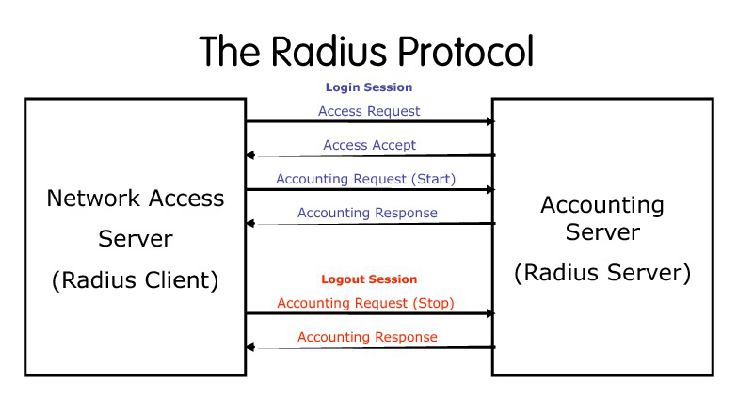
\includegraphics{figure/RADIUS_protocollo.eps}
  \caption{Il protocollo RADIUS}
  \label{RADIUS}
\end{figure}

\subsubsection{Protocollo: messaggi}
La figura \ref{RADIUS_protocollo_messaggi} mostra i messaggi scambiati dal protocollo RADIUS.
\begin{figure}[htbp]
  \centering
  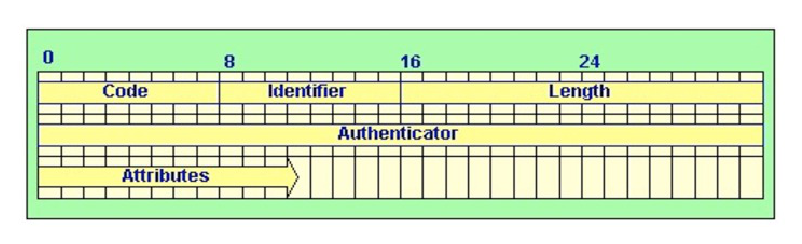
\includegraphics{figure/RADIUS_protocollo_messaggi.eps}
  \caption{Messaggi del protocollo RADIUS}
  \label{RADIUS_protocollo_messaggi}
\end{figure}
\begin{description}
\item [Code:] Il byte che contengono il comando/risposta RADIUS.
\item [Identifier:] Il byte che identifica il comando/risposta RADIUS.
\item [Length:] Lunghezza del pacchetto.
\item [Authenticator:] Valore usato per la risposta del server all'autenticazione RADIUS.
\item [Attributes:] Attributi del comando/risposta.
\end{description}

\subsection{Cattura dei pacchetti}
\subsubsection{libpcap}
Usando la libreria libpcap si fa si che tutti i pacchetti che arrivano alla scheda di rete vengano copiati e inviati al driver BPF (si veda figura  \ref{libpcap_cattura_dei_pacchetti}). Mentre il pacchetto originale segue il naturale percorso e quindi pu� anche essere scartato dalla scheda di rete se l'indirizzo MAC non corrisponde, il pacchetto copiato viene gestito dall'applicazione (quindi con l'ausilio della CPU).

\subsubsection{libpcap: esempio d'uso}

{\footnotesize
\begin{verbatim}
pcapPtr = pcap_open_live(deviceName,
     maxCaptureLen, setPromiscousMode,
     pktDelay, errorBuffer);
while(pcap_dispatch(pcapPtr, 1,
          processPacket, NULL) != -1);
void processPacket(u_char *_deviceId,
     const struct pcap_pkthdr *h,
     const u_char *p) {
     ...
}

int main(int argc, char* argv[]) {
  /* open a network interface */
descr = pcap_open_live(dev,BUFSIZ,0, 1,errbuf);
/* install a filter */
pcap_compile(descr,&fp,"dst port 80",0,netp);
pcap_setfilter(descr,&fp);
while (1) {
    /* Grab packets forever */
    packet = pcap_next(descr,&hdr);
    /* print its length */
    printf("Grabbed packet of length %d\n", hdr.len);
  }
}
\end{verbatim}
}

\begin{figure}[htbp]
  \centering
  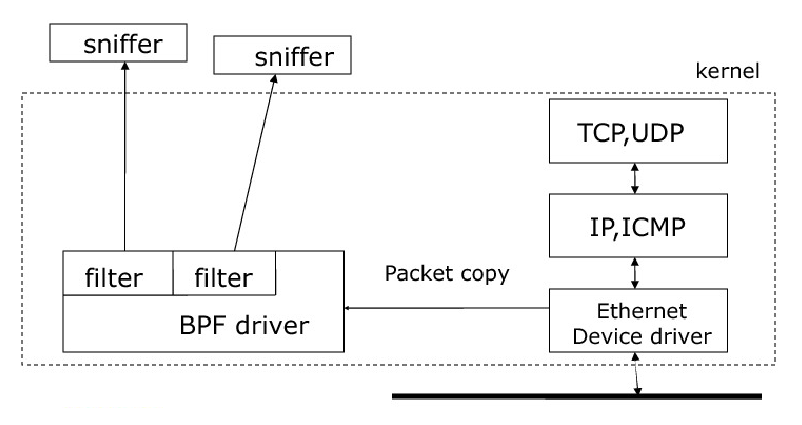
\includegraphics{figure/libpcap_cattura_pacchetti.eps}
  \caption{libpcap: cattura dei pacchetti}
  \label{libpcap_cattura_dei_pacchetti}
\end{figure}

\subsubsection{Problemi comuni con la cattura dei pacchetti}
\begin{itemize}
\item Problemi di sicurezza:
  \begin{itemize}
  \item Viene catturato tutto il traffico di rete e non solo quello destinato all'host che ``sniffa''.
  \item Se c'� una rete switchata viene catturato solo una parte del traffico (\glstext{ARP poisoning}).
  \item L'usabilit� � limitata ha chi ha i privilegi di root\\
    Nota: questo succede anche con il comando ICMP (ad esempio ping) e perci� questo comando ha il setuid abilitato.
  \end{itemize}
\item Performance:
  \begin{itemize}
  \item Lo sniffer implica anche carico di lavoro sulla CPU perch� tutti i pacchetti catturati devono essere analizzati dal programma e non solo quelli diretti verso l'host.
  \end{itemize}
\end{itemize}

\subsubsection{Cattura dei pacchetti: soluzioni}
\begin{itemize}
\item Usare una NIC (Network Interface Cart - scheda di rete) punta sulla NPU (Network Process Unit\footnote{Una Network Process Unit (NPU) � un array di una o pi� CPU specializzate per gestire le funzioni di rete. Le NPU hanno l'obiettivo di esaminare e manipolare in maniera efficiente l'header dei pacchetti.}). Ogni moderna NIC ha un limitato numero di NPU (\glstext{multicast} e ethernet). Se si possiede un driver che sfrutta al meglio la NPU allora si possono fare anche altre cose, oltre al filtraggio per MAC address.
\item Usare una scheda programmabile (ad esempio Napatech, si veda figura \ref{cattura_napatech}).
\item Eseguire il codice di gestione/amministrazione del traffico direttamente sulla NIC (ad esempio Inter IPX Family).
\item Accesso ad alta velocit� (via mmap()) per prendere i pacchetti direttamente dalla NIC via bus PCI (ad esempio Endage DAG Card, si veda figura \ref{cattura_DAG}).
\end{itemize}

\begin{figure}[htbp]
  \centering
  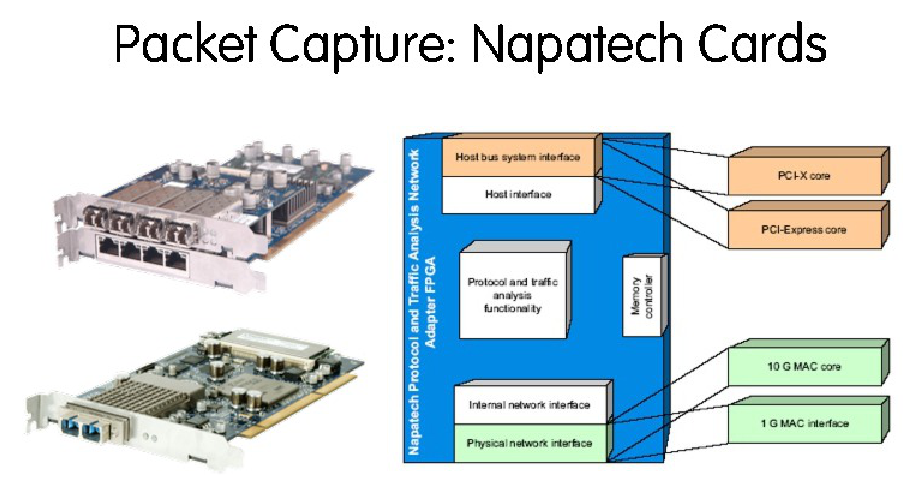
\includegraphics{figure/Network_capture_Napatech.eps}
  \caption{Cattura dei pacchetti: schede di rete Napatech}
  \label{cattura_napatech}
\end{figure}

\begin{figure}[htbp]
  \centering
  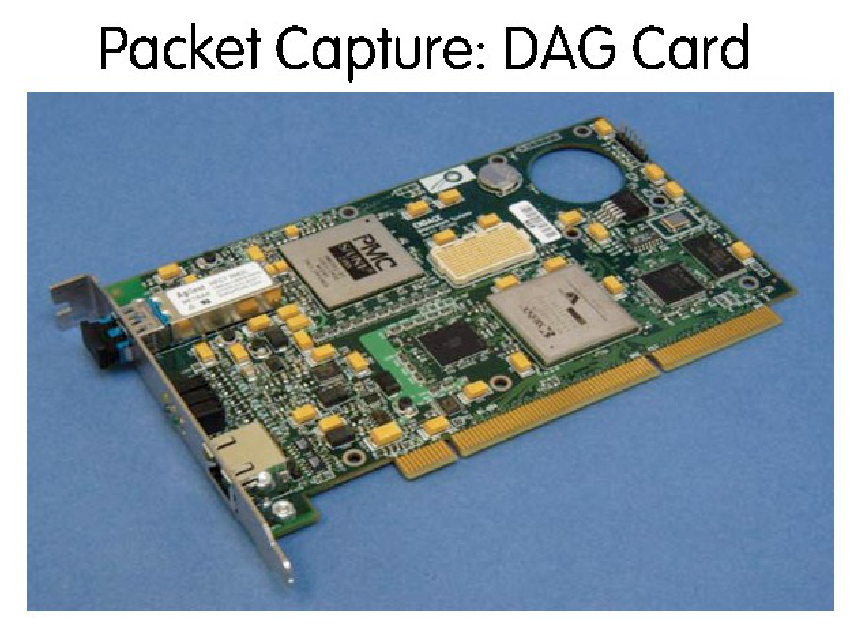
\includegraphics{figure/Network_capture_DAG.eps}
  \caption{Cattura dei pacchetti: scheda di rete DAG}
  \label{cattura_DAG}
\end{figure}

\begin{figure}[htbp]
  \centering
  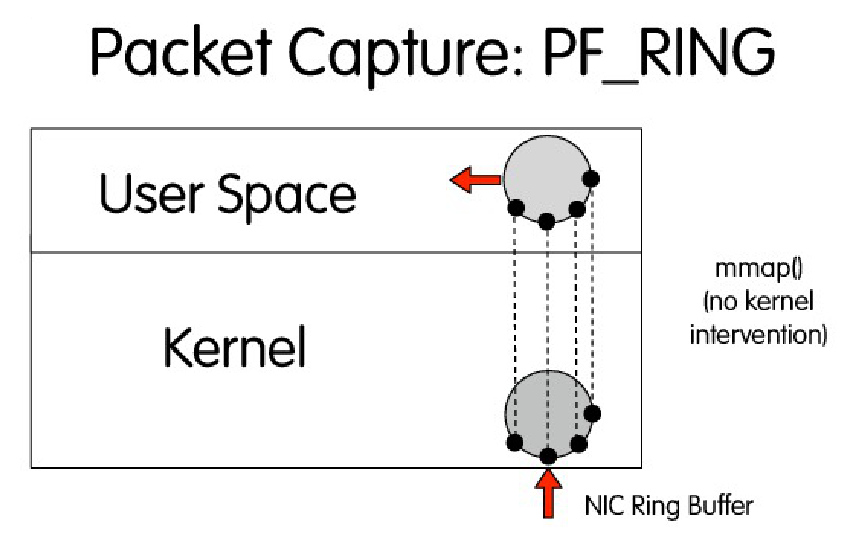
\includegraphics{figure/Network_capture_PF_Ring.eps}
  \caption{Cattura dei pacchetti: PF Ring in DNA (Direct NIC Access) mode}
\end{figure}

\subsection{Mirror del traffico: possibili soluzioni}
Hardware:
\begin{itemize}
\item Hub (ethernet in rame, token ring).
\item Divisione ottica (fibra ottica).
\item Tap (Rame/fibra) (si veda figura \ref{mirror_schede_tap})
\end{itemize}

Software:
\begin{itemize}
\item Switch Port Mirror (1:1, 1:N).
\item Switch VLAN Mirror (N:1).
\item Switch Traffic Filter/Mirroring (Juniper).
\end{itemize}

\begin{figure}[htbp]
  \centering
  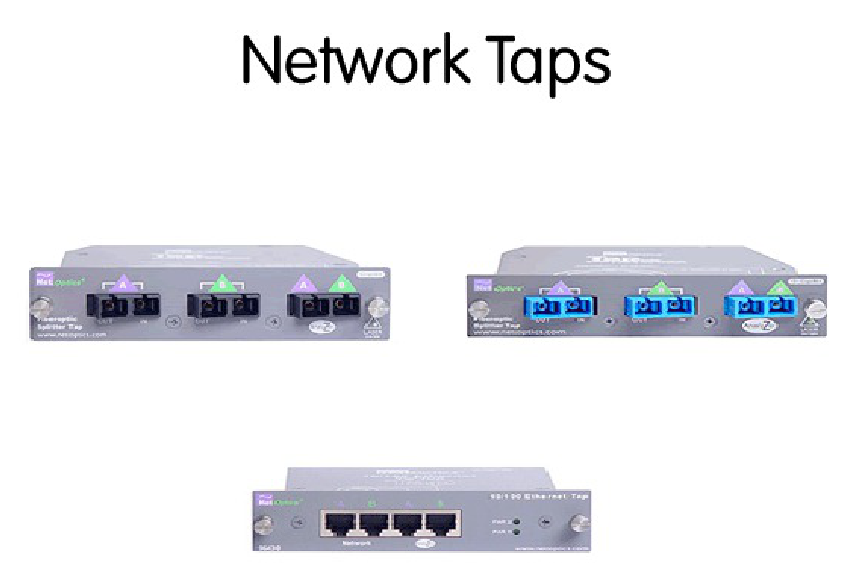
\includegraphics{figure/Network_tap.eps}
  \caption{Mirror del traffico: Tap}
  \label{mirror_schede_tap}
\end{figure}

\subsection{Collezionare i dati: RRD}
\begin{itemize}
\item RRD (\url{http://www.rrdtool.org/})
  \begin{itemize}
  \item Round Robin Database: strumento per scrivere e visualizzare i dati basato su MRTG (Multi Router Traffic Grapher).
  \item I dati sono scritti in un formato ``compresso'' che non aumenta nel tempo (i dati vengono aggregati automaticamente) lasciando inalterata la dimensione del file.
  \item Interfacce Perl/C per accedere ai dati e produrre i grafici.
  \end{itemize}
\end{itemize}

\subsubsection{Esempio in Perl}

{\footnotesize
\begin{verbatim}
$rrd = "$dataDir/$agent-$ifIndex.rrd";
if(! -e $rrd) {
    RRDs::create ($rrd, "--start",$now-1, "--step",20,
      "DS:bytesIn:COUNTER:120:0:10000000",
      "DS:bytesOut:COUNTER:120:0:10000000",
      "RRA:AVERAGE:0.5:3:288");
    $ERROR = RRDs::error;
    die "$0: unable to create `$rrd': $ERROR\n" if $ERROR;
}
    RRDs::update $rrd, "$now:$ifInOctets:$ifOutOctets";
   if ($ERROR = RRDs::error) {
    die "$0: unable to update `$rrd': $ERROR\n";
}
\end{verbatim}
}

\begin{figure}[htbp]
  \centering
  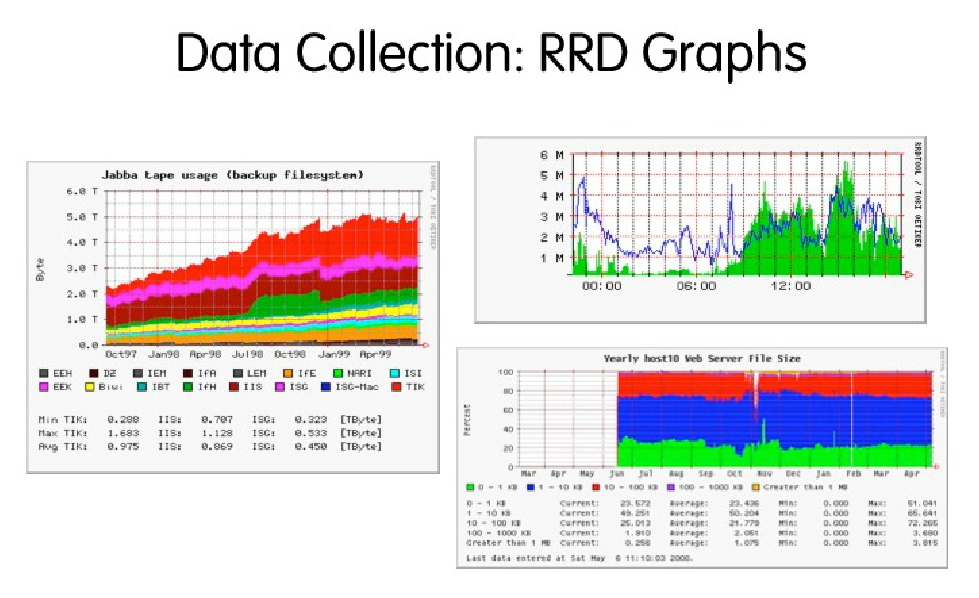
\includegraphics{figure/RRD.eps}
  \caption{Collezionare i dati: RRD}
\end{figure}

% LocalWords:  sFlow collezionatore MIB SNMP RFC InMon Inc UDP NetFlow sniffer
% LocalWords:  GB ntop org Switch Router Multigigabit RADIUS Authentication and
% LocalWords:  Dial Service Rigney Rubens Simpson Willens January Accounting PF
% LocalWords:  wired lines client accounting Access Request Accept Reject CHAP
% LocalWords:  Challenge Response Identifier Length Authenticator Attributes
% LocalWords:  libpcap BPF MAC all'host sniffa' switchata ARP poisoing ICMP NIC
% LocalWords:  setuid l'host Interface Cart NPU Process Unit array l'header IPX
% LocalWords:  multicast ethernet Napatech Family mmap Endage DAG Mirror Hub
% LocalWords:  token Port VLAN Traffic Filter Mirroring Juniper RRD Robin MRTG
% LocalWords:  Grapher Perl

\section{Misurazione del traffico: qualche caso di studio}
\subsection{Caratterizzazione del percorso: patchar}
Pathchar \url{ftp://ftp.ee.lbl.gov/pathchar/}
\begin{itemize}
\item Spedisce vari pacchetti (di differenti dimensioni) verso tutti i router, che devono essere analizzati, di un dato percorso.
\item Misura il tempo di risposta pi� breve per ogni hop:
  \begin{itemize}
  \item Ritardo dell'hop.
  \item Larghezza di banda.
  \item Coda
  \end{itemize}
\item Studia il \gls{RTT} respetto alla dimensione del pacchetto, misura la disponibilit� della larghezza di banda.
\item Svantaggi: il test dura troppo. I calcoli sono complessi e necessitano l'invio di un gran numero di pacchetti per dare misurazioni precise.
\end{itemize}

Altri strumenti: pchar, pipechar.

\subsection{Throughput della rete: Iperf}
Iperf \url{http://dast.nlanr.net/Projects/Iperf/}
\begin{itemize}
\item Architettura client/server: qualche binario viene eseguito in due modi differenti.
\item L'applicazione client spedisce al server pacchetti TCP/UDP. Pu� essere specificata la porta, la durata del test, la dimensione della finestra TCP, il volume dei dati del test.
\item Statistiche: larghezza di banda, perdita/ritardo dei pacchetti, jitter.
\item Svantaggi:
  \begin{itemize}
  \item L'applicazione server deve essere installata sull'host di destinazione.
  \item Non lo si pu� installare/usare sui router.
  \end{itemize}
\end{itemize}

\subsection{Di che tipo di report sul traffico abbiamo bisogno?}
\begin{itemize}
\item La top N dei parlatori (chi trasmette molto traffico).
\item La top N delle conversazioni (le coppie di host che si trasmettono molto traffico).
\item La top N delle applicazioni (ad esempio SAP usa il 70\% della larghezza di banda disponibile).
\item Il volume dei dati per entit� di base (link, locazione, regione, classe di utenti).
\item Volume dei dati e velocit� per \gls{AS} (per sapere ad esempio se si ha bisogno di stipulare un nuovo contratto).
\item Marca \gls{QoS} per le applicazioni o per le entit� di base (ad esempio, il \gls{BGP} pu� dire se si sta spedendo il traffico sul percorso migliore?).
\item Rapporti sul traffico che non ci si aspetta di vedere sulla rete (ad esempio perch� l'host X sta spedendo un pacchetto IPX anche se si parla usando solamente IP?).
\end{itemize}

\subsection{Monitoraggio integrato: Cacti}
Cacti \url{http://www.raxnet.net/products/cacti} � uno strumento open source capace di:
\begin{itemize}
\item Collezionare i dati con l'ausilio di metodi SNMP e altri non-SNMP.
\item La configurazione viene fatta via web e la scrittura su un database MySQL.
\item Statistiche salvate in RRD.
\item Estensibilit� attraverso script e XML.
\end{itemize}

\begin{figure}[htbp]
  \centering
  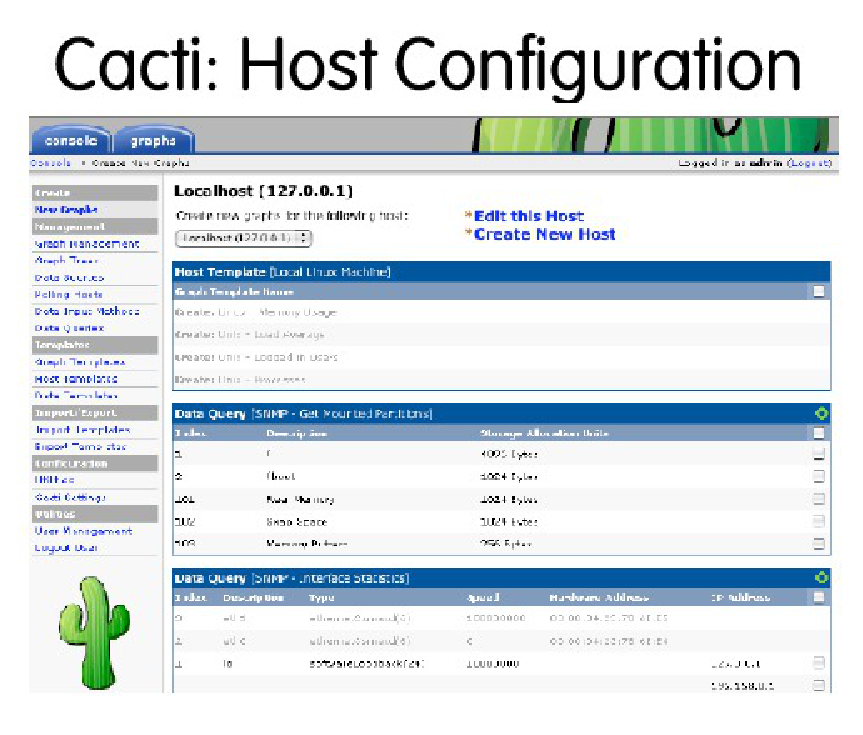
\includegraphics{figure/Cacti_configurazione.eps}
  \caption{Cacti: configurazione}
\end{figure}

\begin{figure}[htbp]
  \centering
  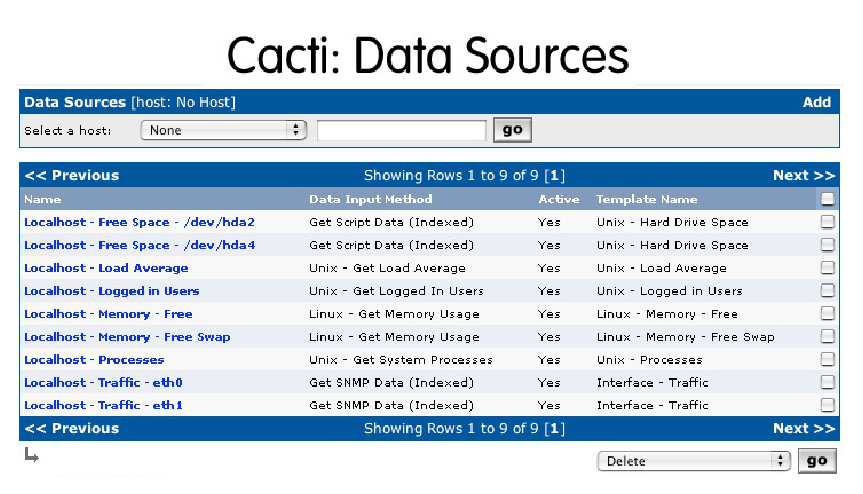
\includegraphics{figure/Cacti_dati.eps}
  \caption{Cacti: dati}
\end{figure}

\begin{figure}[htbp]
  \centering
  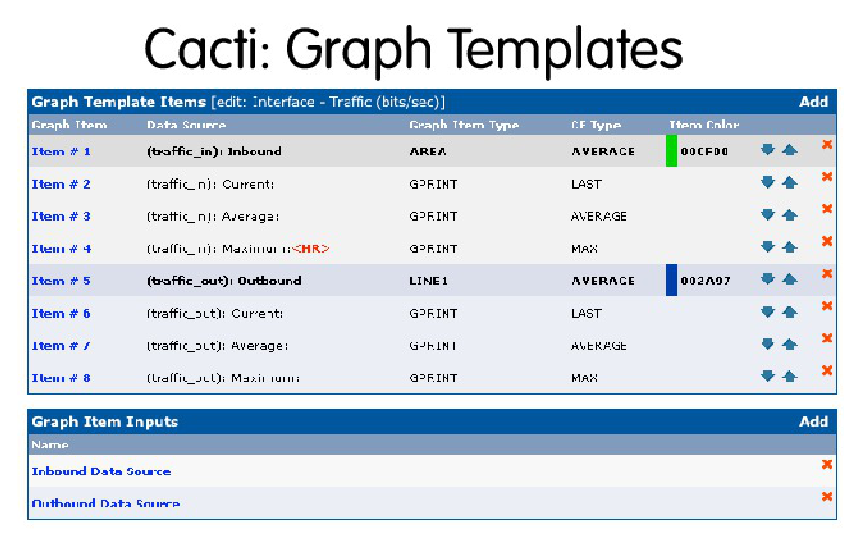
\includegraphics{figure/Cacti_grafico_template.eps}
  \caption{Cacti: grafico dei template}
\end{figure}

\subsection{Caso di studio: gestione della larghezza di banda}
\begin{itemize}
\item I problemi che non sono legati all'acquisto di nuova larghezza di banda ma alla gestione di quella attuale.
  \begin{itemize}
  \item Lezione appresa: pi� larghezza di banda si ha, pi� verr� usata.
  \end{itemize}
  \begin{figure}[htbp]
    \centering
    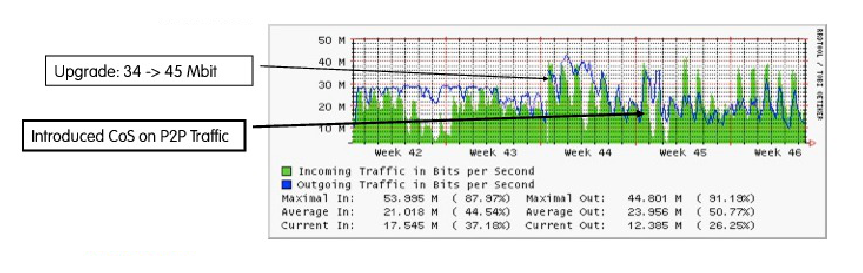
\includegraphics{figure/Gestione_larghezza_di_banda.eps}
    \caption{Gestione della larghezza di banda}
  \end{figure}
\item Soluzione: monitorare e trovare le risposte per le proprie esigenze (non ci sono soluzioni generali).
  \begin{itemize}
  \item Analizzare quanta della larghezza di banda viene utilizzata (ad esempio, perch� viene utilizzato il protocollo X?).
  \item Traffico e matrice del flusso: chi parla con chi e quali dati si scambiano?
  \end{itemize}
\item Lezioni apprese dalla pratica:
  \begin{itemize}
  \item Scarse performance possono essere causate dall'uso dei link di backup perch� quelli primari non sono disponibili (si sta monitorando il failovers - attraverso le trap SNMP - come STP, stato delle porte?).
  \item La rete va bene ma non � al massimo (suboptimal) o � molto dinamica? (SNMP fornisce molti MIB a questo scopo).
  \item Si sta tagliando troppo la banda (shaping\footnote{Lo shaping si effettua introducendo delle classi di servizio (CoS) per impedire che un tipo di traffico monopilizzi tutto.})? Le CoS (Class of Service) sono ottime, ma non se ne dovrebbe abusare (si dovrebbe invece monitorare la quantit� di traffico tagliata dalle proprie politiche)!
  \end{itemize}
\end{itemize}

\subsection{Caso di studio: dov'� un host?}
\begin{itemize}
\item Associazione tra indirizzo IP e nome:
  {\footnotesize
\begin{verbatim}
deri@tar:~$ nslookup 131.114.21.22
   Server: localhost
   Address: 127.0.0.1
   Name: jake.unipi.it
   Address: 131.114.21.22
\end{verbatim}
  }
\item Associazione tra host e proprietario
  \begin{itemize}
  \item namenslookup-type=SOA.
  \item WAIS (Wide Area Information System) \url{http://www.ai.mit.edu/extra/the-net/wais.html}.
  \item  WHOIS [RFC-812].
  \end{itemize}
\end{itemize}

\subsubsection{Esempio di whois}

{\footnotesize
\begin{verbatim}
Domain:         unipi.it
Status:         ACTIVE
Created:        1996-01-29 00:00:00
Last Update:    2008-02-14 00:02:47
Expire Date:    2009-01-29

Registrant
  Name:         Universita' degli Studi di Pisa
  ContactID:    UNIV302-ITNIC
  Address:      Centro SERRA
                Pisa
                56100
                PI
                IT
  Created:      2007-03-01 10:42:01
  Last Update:  2008-01-19 09:46:08

Registrar
  Organization: Consortium GARR
  Name:         GARR-MNT
\end{verbatim}
}

\subsection{Dov'� l'host X nel mondo?}
\begin{itemize}
\item  RFC 1876: un mezzo per Expressing Location Information nel Domain Name System,
\item \url{http://www.caida.org/tools/utilities/netgeo/}
\item \url{http://www.maxmind.com/}
\item \url{http://www.geobytes.com/}
\end{itemize}

\subsection{Caso di studio: impronta digitale degli OS (Operating System - sistema operativo)}
\begin{itemize}
\item Attivo:\\
  Spedire pacchetti di prova per capire il sistema operativo dell'host (\url{http://nmap.org/}).
\item Passivo:\\
  Guardare la stretta di mano a 3 vie (handshake) del TCP e confrontarla con un database di firme conosciute in modo da capire il sistema operativo dell'host (\url{http://ettercap.sf.net/}).
\end{itemize}

\subsubsection{Ettercap}

{\footnotesize
\begin{verbatim}
WWWW:MSS:TTL:WS:S:N:D:T:F:LEN:OS

WWWW: 4 digit hex field indicating the TCP Window Size
MSS : 4 digit hex field indicating the TCP Option Maximum Segment Size
      if omitted in the packet or unknown it is "_MSS"
TTL : 2 digit hex field indicating the IP Time To Live
WS  : 2 digit hex field indicating the TCP Option Window Scale
      if omitted in the packet or unknown it is "WS"
S   : 1 digit field indicating if the TCP Option SACK permitted is true
N   : 1 digit field indicating if the TCP Options contain a NOP
D   : 1 digit field indicating if the IP Don't Fragment flag is set
T   : 1 digit field indicating if the TCP Timestamp is present
F   : 1 digit ascii field indicating the flag of the packet
      S = SYN
      A = SYN + ACK
\end{verbatim}
}

\subsection{Caso di studio: scanner per la sicurezza}
\begin{itemize}
\item Nessus \url{http://www.nessus.org/}.
\item Saint \url{http://www.saintcorporation.com/}.
\end{itemize}

\begin{figure}[htbp]
  \centering
  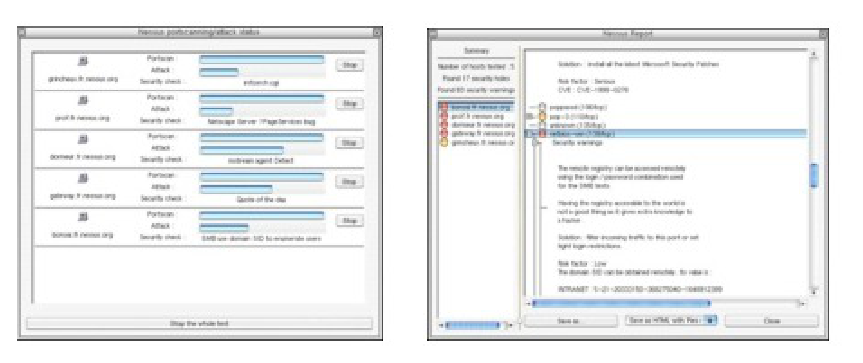
\includegraphics{figure/Scanner_sicurezza.eps}
  \caption{Scanner per la sicurezza}
\end{figure}

\subsection{Caso di studio: sicurezza di rete}
La sicurezza � un processo, non un prodotto (Standard BS 7799, B. Schneier).
\begin{itemize}
\item Si � capaci di determinare le anomalie del traffico?
\item Si � sicuri di sapere cosa monitorare? Molti problemi sono prodotti dal traffico che non ci si aspetta di vedere sulla rete: monitorare ogni cosa, filtrare solo quello che dovrebbe passare, vedere il resto e spiegarsi cos'� successo.
\item Si possiede un meccanismo automatico per recuperare i fallimenti? Si supponga di aver individuato un problema (ad esempio attraverso le trap SNMP) il sistema � capace di reagire in maniera automatica o si deve aspettare il rientro dell'amministratore dalle vacanze?
\end{itemize}

\subsection{Caso di studio: individuazione del traffico \glsentrytext{P2P}}
\begin{itemize}
\item Il \gls{P2P} � difficile da individuare con i metodo classici:
  \begin{itemize}
  \item Non lo si pu� individuare attraverso l'uso di impronte digitali (ad esempio con l'associazione porta-protocollo).
  \end{itemize}
\item Comunque:
  \begin{itemize}
  \item Lo si pu� individuare in termini di modifica di un comportamento standard (ad esempio una workstation non pu� aprire pi� di X connessioni al minuto, e non pu� nemmeno avere pi� di Y connessioni aperte).
  \item Analizzare una parte iniziale del payload per individuare il protocollo.
  \item Alta percentuale di connessione TCP fallite.
  \item Il rapporto pacchetti/byte e sopra la media (le sorgenti \gls{P2P} spediscono molti pacchetti, per lo pi� per parlare con i peer).
  \item Identificare l'esistenza di comunicazione client-a-client (porte $>$ alla 1024) anche se non si hanno canali di comunicazione FTP aperti.
  \end{itemize}
\end{itemize}

\subsection{Caso di studio: individuazione dello SPAM}
\begin{itemize}
\item Reti grandi e aperte (come Universit� o \gls{ISP}) sono il posto migliore dove inviare SPAM (email non richieste).
\item Come identificare la sorgente di SPAM:
  \begin{itemize}
  \item Problema simile all'individuazione del traffico \gls{P2P} ma pi� semplice (solo SMTP, 1 connessione = 1 email).
  \item Selezionare l'insieme dei top N mittenti SMTP.
  \item Rimuovere dall'insieme tutti i server SMTP conosciuti.
  \item Gli studi mostrano che in media gli host non inviano pi� di 8-10 email al minuto.
  \item Un problema veramente semplice da affrontare usando dei protocolli basati sui flusso, come ad esempio NetFlow.
  \end{itemize}
\end{itemize}

\subsection{Caso di studio: individuazione dei virus/trojan}
\begin{itemize}
\item Problema simile all'individuazione dello SPAM ma pi� complesso dato che i protocolli e le porte usate non sono fisse.
\item Gli attacchi non hanno obiettivi mirati: in qualche modo si comportano come scanner di rete.
\item Individuazione:
  \begin{itemize}
  \item Se il problema � conosciuto (ad esempio il traffico sulla porta UDP 135) ci si focalizza su questi traffici.
  \item Buttare un occhio ai messaggi ICMP (ad esempio porta o destinazione non raggiungibile) sono il modo migliore per individuare gli scanner di rete.
  \end{itemize}
\end{itemize}

% LocalWords:  patchar Pathchar router hop dell'hop RTT Trip pchar pipechar TCP
% LocalWords:  Throughput Iperf client UDP jitter sull'host report host SAP AS
% LocalWords:  QoS BGP l'host IPX Cacti source SNMP MySQL RRD template trap STP
% LocalWords:  failovers suboptimal MIB shaping CoS Class of Service type SOA
% LocalWords:  namenslookup WAIS Wide Information System WHOIS RFC whois Domain
% LocalWords:  Expressing Location Name OS Operating dell'host handshake Nessus
% LocalWords:  Ettercap BS Schneier payload peer FTP SPAM SMTP NetFlow trojan
% LocalWords:  ICMP

\section{Commenti finali}
\subsection{Quindi, cosa bisogna aspettarsi dal monitoraggio di rete?}
\begin{itemize}
\item Capacit� di individuare in maniera automatica quei problemi che sono costantemente sotto monitoraggio (ad esempio, non c'� traffico su di un link della backbone: la rete � caduta?).
\item Ricevere allarmi a proposito di potenziali (ad esempio l'utilizzo della CPU � troppo alto) e reali (ad esempio li disco � pieno) problemi.
\item Notifica e ripristino automatico di problemi noti con note soluzioni (ad esempio, se il link dell'email non va viene usato un link di backup).
\item Notificare all'uomo tutti quei problemi che necessitano attenzione e che non possono essere ripristinati (ad esempio l'host X non � raggiungibile).
\end{itemize}

\subsection{Avvertenze sul monitoraggio}
\begin{itemize}
\item Se un'applicazione necessita di assistenza umana per quei problemi che possono essere risolti in maniera automatica, allora l'uso di questa applicazione non � completamente vantaggioso.
\item Gli allarmi (sicurezza al 100\% che c'� qualcosa che non va) sono diversi dagli avvisi (potrebbe esserci qualche problema): non si pretenda di essere precisi/catastrofici se non � il caso.
\item Gli allarmi sono inutili se non c'� nessuno che li controlla.
\item Troppi (falsi) allarmi equivale a non avere allarmi: gli umani tendono ad ignorare i fatti quando qualcuno di essi � falso.
\end{itemize}

% LocalWords:  backbone l'host


% Il glossario
\newpage
\pagenumbering{roman}
\printglossary[style=altlistgroup]

\end{document}
